%%%%%%%%%%%%%%%%%%%%%%%%%%%%%%%%%%%%%%%%
% Bazirano na FRI predlogi

\documentclass[a4paper, 12pt, openright]{book}
% \documentclass[a4paper, 12pt, openright, draft]{book}
% Nalogo preverite tudi z opcijo draft, ki pokaže, katere vrstice so predolge! Pozor, v draft opciji, se slike ne pokažejo!

% \usepackage[a-1b]{pdfx}
% \hypersetup{pdftex, colorlinks=true, citecolor=black, filecolor=black, linkcolor=black, urlcolor=black, pdfproducer={LaTeX}, pdfcreator={LaTeX}}

\usepackage[utf8]{inputenc}   % omogoča uporabo slovenskih črk kodiranih v formatu UTF-8
\usepackage[slovene, english]{babel}    % naloži, med drugim, slovenske delilne vzorce
\usepackage[pdftex]{graphicx}  % omogoča vlaganje slik različnih formatov
\usepackage{fancyhdr}          % poskrbi, na primer, za glave strani
\usepackage{amssymb}           % dodatni matematični simboli
\usepackage{amsmath}           % eqref, npr.
\usepackage[hyphens]{url}
\usepackage{csquotes}
\usepackage{enumitem}
\usepackage{float}
% \usepackage{stmaryrd}
\usepackage{caption}
\usepackage[
    pdftex,
    colorlinks=true,
	citecolor=black,
    filecolor=black,
    linkcolor=black,
    urlcolor=black,
	pdfproducer={LaTeX},
    pdfcreator={LaTeX}
]{hyperref}
\usepackage{hyperxmp}
\usepackage{color}
\usepackage{soul}
\usepackage[
    backend=biber,
    style=numeric,
    sorting=nty,
]{biblatex}
\usepackage{listings}
\usepackage{xcolor}

% Imports bibliography file
\addbibresource{literatura.bib}

%%%%%%%%%%%%%%%%%%%%%%%%%%%%%%%%%%%%%%%%
%	DIPLOMA INFO
%%%%%%%%%%%%%%%%%%%%%%%%%%%%%%%%%%%%%%%%
\newcommand{\ttitle}{Pohitritev aplikacij z vzorcem matrice z uporabo grafičnih procesnih enot}
\newcommand{\ttitleEn}{Accelerating stencil applications on graphics processing units}
\newcommand{\tsubject}{\ttitle}
\newcommand{\tauthor}{Tadej Vengust}
\newcommand{\tkeywords}{GPE, Nvidia, CUDA, matrica, Lenia}
\newcommand{\tkeywordsEn}{GPU, Nvidia, CUDA, stencil, Lenia}

%%%%%%%%%%%%%%%%%%%%%%%%%%%%%%%%%%%%%%%%
%	HYPERREF SETUP
%%%%%%%%%%%%%%%%%%%%%%%%%%%%%%%%%%%%%%%%
\hypersetup{pdftitle={\ttitle}}
\hypersetup{pdfsubject=\ttitleEn}
\hypersetup{pdfauthor={\tauthor}}
\hypersetup{pdfkeywords=\tkeywordsEn}

%%%%%%%%%%%%%%%%%%%%%%%%%%%%%%%%%%%%%%%%
% postavitev strani
%%%%%%%%%%%%%%%%%%%%%%%%%%%%%%%%%%%%%%%%

% robovi za tisk
\addtolength{\marginparwidth}{-20pt}
\addtolength{\oddsidemargin}{40pt}
\addtolength{\evensidemargin}{-40pt}

\renewcommand{\baselinestretch}{1.3} % ustrezen razmik med vrsticami
\setlength{\headheight}{15pt}        % potreben prostor na vrhu
\renewcommand{\chaptermark}[1]
{\markboth{\MakeUppercase{\thechapter.\ #1}}{}} \renewcommand{\sectionmark}[1]
{\markright{\MakeUppercase{\thesection.\ #1}}} \renewcommand{\headrulewidth}{0.5pt} \renewcommand{\footrulewidth}{0pt}
\fancyhf{}
\fancyhead[LE,RO]{\sl \thepage}
%\fancyhead[LO]{\sl \rightmark} \fancyhead[RE]{\sl \leftmark}
\fancyhead[RE]{\sc \tauthor}
\fancyhead[LO]{\sc Diplomska naloga}


\newcommand{\BibLaTeX}{{\sc Bib}\LaTeX}
\newcommand{\BibTeX}{{\sc Bib}\TeX}

%%%%%%%%%%%%%%%%%%%%%%%%%%%%%%%%%%%%%%%%
% naslovi
%%%%%%%%%%%%%%%%%%%%%%%%%%%%%%%%%%%%%%%%

\newcommand{\autfont}{\Large}
\newcommand{\titfont}{\LARGE\bf}
\newcommand{\clearemptydoublepage}{\newpage{\pagestyle{empty}\cleardoublepage}}
\setcounter{tocdepth}{2}	      % globina kazala

%%%%%%%%%%%%%%%%%%%%%%%%%%%%%%%%%%%%%%%%
% konstrukti
%%%%%%%%%%%%%%%%%%%%%%%%%%%%%%%%%%%%%%%%
\newtheorem{izrek}{Izrek}[chapter]
\newtheorem{trditev}{Trditev}[izrek]
\newenvironment{dokaz}{\emph{Dokaz.}\ }{\hspace{\fill}{$\Box$}}

% \newfloat{graph}{htbp}{log}
% \floatname{graph}{Graf}
% \captionsetup[graph]{position=top}

\captionsetup[table]{position=top}

% \newfloat{table}{htbp}{log}
% \floatname{table}{Tabela}
% \captionsetup[table]{position=top}

% Listing -> Izsek kode
\renewcommand{\lstlistingname}{Izsek kode}

%%%%%%%%%%%%%%%%%%%%%%%%%%%%%%%%%%%%%%%%%%%%%%%%%%%%%%%%%%%%%%%%%%%%%%%%%%%%%%%
%% PDF-A
%%%%%%%%%%%%%%%%%%%%%%%%%%%%%%%%%%%%%%%%%%%%%%%%%%%%%%%%%%%%%%%%%%%%%%%%%%%%%%%

%%%%%%%%%%%%%%%%%%%%%%%%%%%%%%%%%%%%%%%%
% define medatata
%%%%%%%%%%%%%%%%%%%%%%%%%%%%%%%%%%%%%%%%
\def\Title{\ttitle}
\def\Author{\tauthor, tv6864@student.uni-lj.si}
\def\Subject{\ttitleEn}
\def\Keywords{\tkeywordsEn}

%%%%%%%%%%%%%%%%%%%%%%%%%%%%%%%%%%%%%%%%
% \convertDate converts D:20080419103507+02'00' to 2008-04-19T10:35:07+02:00
%%%%%%%%%%%%%%%%%%%%%%%%%%%%%%%%%%%%%%%%
\def\convertDate{
    \getYear
}

{\catcode`\D=12
 \gdef\getYear D:#1#2#3#4{\edef\xYear{#1#2#3#4}\getMonth}
}
\def\getMonth#1#2{\edef\xMonth{#1#2}\getDay}
\def\getDay#1#2{\edef\xDay{#1#2}\getHour}
\def\getHour#1#2{\edef\xHour{#1#2}\getMin}
\def\getMin#1#2{\edef\xMin{#1#2}\getSec}
\def\getSec#1#2{\edef\xSec{#1#2}\getTZh}
\def\getTZh +#1#2{\edef\xTZh{#1#2}\getTZm}
\def\getTZm '#1#2'{
    \edef\xTZm{#1#2}
    \edef\convDate{\xYear-\xMonth-\xDay T\xHour:\xMin:\xSec+\xTZh:\xTZm}
}

%\expandafter\convertDate\pdfcreationdate

%%%%%%%%%%%%%%%%%%%%%%%%%%%%%%%%%%%%%%%%
% get pdftex version string
%%%%%%%%%%%%%%%%%%%%%%%%%%%%%%%%%%%%%%%%
\newcount\countA
\countA=\pdftexversion
\advance \countA by -100
\def\pdftexVersionStr{pdfTeX-1.\the\countA.\pdftexrevision}


%%%%%%%%%%%%%%%%%%%%%%%%%%%%%%%%%%%%%%%%
% XMP data
%%%%%%%%%%%%%%%%%%%%%%%%%%%%%%%%%%%%%%%%
\usepackage{xmpincl}
% \includexmp{pdfa-1b}

%%%%%%%%%%%%%%%%%%%%%%%%%%%%%%%%%%%%%%%%
% pdfInfo
%%%%%%%%%%%%%%%%%%%%%%%%%%%%%%%%%%%%%%%%
\pdfinfo{
    /Title    (\ttitle)
    /Author   (\tauthor, tv6864@student.uni-lj.si)
    /Subject  (\ttitleEn)
    /Keywords (\tkeywordsEn)
    /ModDate  (\pdfcreationdate)
    /Trapped  /False
}

%%%%%%%%%%%%%%%%%%%%%%%%%%%%%%%%%%%%%%%%
% znaki za copyright stran
%%%%%%%%%%%%%%%%%%%%%%%%%%%%%%%%%%%%%%%%

\newcommand{\CcImageCc}[1]{
	
\includegraphics[scale=#1]{cc_cc_30.pdf}
}
\newcommand{\CcImageBy}[1]{
	
\includegraphics[scale=#1]{cc_by_30.pdf}
}
\newcommand{\CcImageSa}[1]{
	
\includegraphics[scale=#1]{cc_sa_30.pdf}
}

%%%%%%%%%%%%%%%%%%%%%%%%%%%%%%%%%%%%%%%%%%%%%%%%%%%%%%%%%%%%%%%%%%%%%%%%%%%%%%%
%%%%%%%%%%%%%%%%%%%%%%%%%%%%%%%%%%%%%%%%%%%%%%%%%%%%%%%%%%%%%%%%%%%%%%%%%%%%%%%

\begin{document}
\selectlanguage{slovene}
\frontmatter
\setcounter{page}{1}
\renewcommand{\thepage}{}       % preprečimo težave s številkami strani v kazalu

%%%%%%%%%%%%%%%%%%%%%%%%%%%%%%%%%%%%%%%%
%naslovnica
 \thispagestyle{empty}
   \begin{center}
    {\large\sc Univerza v Ljubljani\\
%      Fakulteta za elektrotehniko\\% za študijski program Multimedija
%      Fakulteta za upravo\\% za študijski program Upravna informatika
      Fakulteta za računalništvo in informatiko\\
%      Fakulteta za matematiko in fiziko\\% za študijski program Računalništvo in matematika
     }
    \vskip 10em%
    {\autfont \tauthor\par}%
    {\titfont \ttitle \par}%
    {\vskip 3em \textsc{DIPLOMSKO DELO\\[5mm]
%    VISOKOŠOLSKI STROKOVNI ŠTUDIJSKI PROGRAM\\ PRVE STOPNJE\\ RAČUNALNIŠTVO IN INFORMATIKA}\par}%
     UNIVERZITETNI  ŠTUDIJSKI PROGRAM\\ PRVE STOPNJE\\ RAČUNALNIŠTVO IN INFORMATIKA}\par}%
%    INTERDISCIPLINARNI UNIVERZITETNI\\ ŠTUDIJSKI PROGRAM PRVE STOPNJE\\ MULTIMEDIJA}\par}%
%    INTERDISCIPLINARNI UNIVERZITETNI\\ ŠTUDIJSKI PROGRAM PRVE STOPNJE\\ UPRAVNA INFORMATIKA}\par}%
%    INTERDISCIPLINARNI UNIVERZITETNI\\ ŠTUDIJSKI PROGRAM PRVE STOPNJE\\ RAČUNALNIŠTVO IN MATEMATIKA}\par}%
    \vfill\null
% izberite pravi habilitacijski naziv mentorja!
    {\large \textsc{Mentor}: prof. dr. Uroš Lotrič\par}
    {\vskip 2em \large Ljubljana, \the\year \par}
\end{center}
% prazna stran
%\clearemptydoublepage
% izjava o licencah itd. se izpiše na hrbtni strani naslovnice

%%%%%%%%%%%%%%%%%%%%%%%%%%%%%%%%%%%%%%%%
%copyright stran
%%%%%%%%%%%%%%%%%%%%%%%%%%%%%%%%%%%%%%%%
\newpage
\thispagestyle{empty}

\vspace*{5cm}
{\small \noindent
To delo je ponujeno pod licenco \textit{Creative Commons Priznanje avtorstva-Deljenje pod enakimi pogoji 4.0 Slovenija}.
%(ali novej\v so razli\v cico).
To pomeni, da se tako besedilo, slike, grafi in druge sestavine dela kot tudi rezultati diplomskega dela lahko prosto distribuirajo,
reproducirajo, uporabljajo, priobčujejo javnosti in predelujejo, pod pogojem, da se jasno in vidno navede avtorja in naslov tega
dela in da se v primeru spremembe, preoblikovanja ali uporabe tega dela v svojem delu, lahko distribuira predelava le pod
licenco, ki je enaka tej.
Podrobnosti licence so dostopne na spletni strani \href{http://creativecommons.si}{creativecommons.si} ali na Inštitutu za
intelektualno lastnino, Streliška 1, 1000 Ljubljana.

\vspace*{1cm}
\begin{center}  % 0.66 / 0.89 = 0.741573033707865
\CcImageCc{0.741573033707865}\hspace*{1ex}\CcImageBy{1}\hspace*{1ex}\CcImageSa{1}
\end{center}
}

\vspace*{1cm}
{\small \noindent
Izvorna koda diplomskega dela, njeni rezultati in v ta namen razvita programska oprema je ponujena pod licenco GNU General Public License,
različica 3. To pomeni, da se lahko prosto distribuira in/ali predeluje pod njenimi pogoji.
Podrobnosti licence so dostopne na spletni strani \url{http://www.gnu.org/licenses/}.
}

\vfill
\begin{center}
\ \\ \vfill
{\em
Besedilo je oblikovano z urejevalnikom besedil \LaTeX.}
\end{center}

% prazna stran
\clearemptydoublepage

%%%%%%%%%%%%%%%%%%%%%%%%%%%%%%%%%%%%%%%%
% stran 3 med uvodnimi listi
\thispagestyle{empty}
\
\vfill

\bigskip
\noindent\textbf{Kandidat:} Tadej Vengust

\noindent\textbf{Naslov:} \ttitle

% vstavite ustrezen naziv študijskega programa!
\noindent\textbf{Vrsta naloge:} Diplomska naloga na univerzitetnem programu prve stopnje Računalništvo in informatika

% izberite pravi habilitacijski naziv mentorja!
\noindent\textbf{Mentor:} prof. dr. Uroš Lotrič

\bigskip
\noindent\textbf{Opis:}\\
Aplikacije z vzorcem matrice so široko uporabljene v znanstvenih in industrijskih aplikacijah.
Mednje spadajo tudi celični avtomati.
Za pohitritev takih aplikacij z grafičnimi procesnimi enotami obstaja več tehnik.
V diplomskem delu na primeru celičnega avtomata Lenie poiščite in ovrednotite učinkovitost različnih načinov sinhronizacije mreže, domen niti in strategij predpomnjenja v dveh in treh dimenzijah.

\bigskip
\noindent\textbf{Title:} \ttitleEn

\bigskip
\noindent\textbf{Description:}\\
Stencil applications are widely used in scientific and industrial applications.
These also include cellular automata.
There are multiple techniques for accelerating such applications with graphics processing units.
In this diploma thesis, using the Lenia cellular automaton as an example, identify and evaluate the effectiveness of different grid synchronization methods, thread domains, and caching strategies in two and three dimensions.

\vfill



\vspace{2cm}

% prazna stran
\clearemptydoublepage

% zahvala
\thispagestyle{empty}\mbox{}\vfill\null\it
\noindent
% Na tem mestu zapišite, komu se zahvaljujete za pomoč pri izdelavi diplomske naloge oziroma pri vašem študiju nasploh. Pazite, da ne boste koga pozabili. Utegnil vam bo zameriti. Temu se da izogniti tako, da celotno zahvalo izpustite.
Zahvaljujem se prof. dr. Urošu Lotriču za mentorstvo, Evi za podporo in Matevžu za lektoriranje.
\rm\normalfont

% prazna stran
\clearemptydoublepage

%%%%%%%%%%%%%%%%%%%%%%%%%%%%%%%%%%%%%%%%
% posvetilo, če sama zahvala ne zadošča :-)
\thispagestyle{empty}\mbox{}{\vskip0.20\textheight}\mbox{}\hfill\begin{minipage}{0.55\textwidth}
Delo je posvečeno mami.
\normalfont\end{minipage}

% prazna stran
\clearemptydoublepage


%%%%%%%%%%%%%%%%%%%%%%%%%%%%%%%%%%%%%%%%
% kazalo
\pagestyle{empty}
\def\thepage{}  % preprečimo težave s številkami strani v kazalu
\tableofcontents{}
% \listoffigures{}


% prazna stran
\clearemptydoublepage

%%%%%%%%%%%%%%%%%%%%%%%%%%%%%%%%%%%%%%%%
% seznam kratic

% \chapter*{Seznam uporabljenih kratic}

% % po potrebi razširi prvo kolono tabele na račun drugih dveh!
% \noindent\begin{tabular}{p{0.13\textwidth}|p{.38\textwidth}|p{.39\textwidth}}
%     {\bf kratica} & {\bf angleško} & {\bf slovensko} \\ \hline
%     {\bf GPE} & graphics processing unit & grafična procesna enota \\
%     {\bf GPGPU} & general purpose graphics processing unit & splošno namenska grafična procesna enota \\
%     {\bf CPE} & central processing unit & centralna procesna enota \\
%     {\bf CUDA} & compute unified device architecture & računsko enotna arhitektura naprav  \\
%     {\bf SIMT} & single instruction multiple threads & en ukaz, več niti \\
%     {\bf API} & application programming interface & vmesnik za aplikacijsko programiranje \\
%     {\bf SWiC} & scatter without write conflict & razprševanje brez pisalnih konfliktov \\
%     {\bf GoL} & (Conway's) game of life & (Conwayeva) igra življenja \\
%     {\bf SP} & streaming processor & pretočna procesorska enota \\
%     {\bf SM} & streaming multiprocessor & pretočni multiprocesor \\
%     {\bf ALE} & arithmetic logic unit & aritmetično logična enota \\
%     {\bf ISL} & iterative stencil loop & iterativna matrična zanka \\
%     {\bf CA} & cellular automaton & celični avtomat \\
% \end{tabular}


% prazna stran
\clearemptydoublepage

%%%%%%%%%%%%%%%%%%%%%%%%%%%%%%%%%%%%%%%%
% povzetek
\phantomsection
\addcontentsline{toc}{chapter}{Povzetek}
\chapter*{Povzetek}

\noindent\textbf{Naslov:} \ttitle
\bigskip

\noindent\textbf{Avtor:} \tauthor
\bigskip

% \noindent\textbf{Povzetek:}
\noindent
Obstaja več različnih metod optimizacije aplikacij z vzorcem matrice.
Med aplikacije, ki so osnovane na matricah sodijo na primer fizikalne simulacije kot so simulacije v vetrovniku, simulacije elektromagnetizma in turbin ter celični avtomati.
Matrica je v konteksu slednjih skupek urejenih točk v soseščini iskane točke, na podlagi katerih lahko izračunamo stanje točke za vsak časovni korak. Ker je soseščina vedno enaka, govorimo o vzorcu matrice.
V diplomski nalogi smo s pomočjo ogrodja CUDA na celičnem avtomatu Lenia raziskali učinkovitost različnih metod optimizacije izvajanja aplikacij z vzorcem matrice na grafičnih procesnih enotah.
Specifično smo se osredotočali na dvodimenzionalne in trodimenzionalne mreže, na različne velikosti soseščin in na različne načine predpomnjenja.
Diplomska naloga skupaj z rezultati predstavlja osnovo za nadaljnje raziskave na tem področju.
\bigskip

\noindent\textbf{Ključne besede:} \tkeywords.
% prazna stran
\clearemptydoublepage

%%%%%%%%%%%%%%%%%%%%%%%%%%%%%%%%%%%%%%%%
% abstract
\phantomsection
\selectlanguage{english}
\addcontentsline{toc}{chapter}{Abstract}
\chapter*{Abstract}

\noindent\textbf{Title:} \ttitleEn
\bigskip

\noindent\textbf{Author:} \tauthor
\bigskip

% \noindent\textbf{Abstract:}
\noindent
There are several different methods for optimizing stencil applications.
Stencil applications include, for example, physics simulations such as wind tunnel simulations, simulations of electromagnetism and turbines, as well as cellular automata.
In the context of cellular automata, a stencil is a set of ordered points in the neighborhood of a target point, based on which the state of that point can be computed for each time step.
Since the neighborhood is always the same, we refer to this as a stencil pattern.
In this work, we used the CUDA framework and Lenia cellular automaton to research efficiency of different methods of optimization of running stencil applications on graphics processing units.
In particular, we focused on computations on two-dimensional and three-dimensional grids, examining different neighborhood sizes and caching strategies.
This work and its results provide a foundation for further research in this area.
\bigskip

\noindent\textbf{Keywords:} \tkeywordsEn.
\selectlanguage{slovene}
% prazna stran
\clearemptydoublepage

%%%%%%%%%%%%%%%%%%%%%%%%%%%%%%%%%%%%%%%%
\mainmatter
\setcounter{page}{1}
\pagestyle{fancy}

\chapter{Uvod}

Grafične procesne enote (GPE) so v zadnjih nekaj desetletjih doživele ogromen preskok v zmogljivosti, kar je še posebej izrazito v primerjavi z razvojem centralnih procesnih enot (CPE) \cite{Surina_2009}.
Poleg tega so GPE, predvsem zaradi inovacij podjetja Nvidia z ogrodjem CUDA (angl. \textit{compute unified device architecture}), postale tudi primerne za splošno namensko računanje, še posebej za matrične operacije.

Med aplikacije, ki so primerne za računanje na GPE, sodijo tudi aplikacije z vzorcem matrice.
Primeri takih so aplikacije, kjer numerično rešujemo diferenciale enačbe ter celični avtomati.
Oboje se intenzivno uporablja v znanstvenih in industrijskih aplikacijah (na primer pri  simulacijah vetrovnikov, turbin, elektromagnetizma, seizmičnih valov).
Gre torej za simulacije realnih problemov, kjer sta prostor in čas diskretizirana.
Prostor postane mreža celic, vsaka izmed njih je v vsakem časovnem trenutku v stanju, ki ga izračunamo glede na stanje celic iz njene soseščine.
Matrica (angl. \textit{stencil}) je urejena soseščina točke, katere stanje želimo posodobiti. Matrica izpostavi le za računanje relevantne celice in vrednosti. Ker isto soseščino uporabimo za celotno mrežo, takim aplikacijam pravimo, da imajo vzorec matrice.

V literaturi \cite{anjum2022efficient, 10.1145/1513895.1513905, SCHAFER20112027} je mogoče zaslediti več različnih pristopov optimizacije takih aplikacij.
Z večanjem dimenzionalnosti mreže aplikacije in večanjem soseščine matric se povečujeta tudi računska in časovna zahtevnost.

GPE nam omogočajo različne načine za pohitritev programske kode. Med najpomembnejše elemente štejemo skupni pomnilnik.

V diplomski nalogi se osredotočamo na merjenje in analizo zmogljivosti aplikacij z vzorcem matrice glede na različne dejavnike.
Mednje spadajo širina soseščine matrice, dimenzionalnost mreže, različni načini sinhronizacije mreže ter predpomnjenja.
Za implementacijo in testiranje različnih konfiguracij smo uporabili zvezni celični avtomat Lenia \cite{lenia_expanded, lenia}.

V nadaljevanju bomo najprej v prvem delu, \ref{pregled} Pregled področja in sorodna dela, predstavili zgradbo GPE in zasnovo ogrodja CUDA tako iz vidika strojne opreme, kot tudi iz vidika programske abstrakcije.
Poleg tega bomo razložili tudi pomen vzorca matrice in celičnega avtomata Lenia ter povzeli nekaj del iz področja optimizacije aplikacij z vzorcem matrice na GPE.
Za tem bomo v drugem delu, \ref{metodologija} Metodologija in orodja, predstavili in obrazložili podrobnosti naše implementacije, za meritve relevantne parametre ter način izvajanja meritev.
Rezultate bomo predstavili v tretjem delu, \ref{rezultati} Rezultati in razprava, v obliki diagramov in tabel, ločeno po dimenzionalnosti in načinu sinhronizacije mreže.
Za konec bomo predstavili glavne ugotovitve ter predložili ideje za nadaljnje raziskave.

\chapter{Pregled področja in sorodna dela}
\label{pregled}

\section{Grafične procesne enote in CUDA}
\label{gpus}
\raggedbottom

GPE so zaradi svoje grafične zasnove, v primerjavi s CPE bolj učinkovite pri več tipih nalog.
Mednje sodijo problemi z veliko podatkovnega paralelizma in z neodvisnimi podnalogami, na primer matrične operacije \cite{Surina_2009}.

CUDA (angl. \textit{compute unified device architecture}) je platforma za vzporedno računanje in programsko ogrodje, ki omogoča uporabo GPE za splošno namensko računanje, od koder izhaja tudi pojem GPGPU (angl. \textit{general purpose graphics processing unit}).
CUDA je izdelek tehnološkega podjetja Nvidia in zaprtokodna programska oprema lastniškega tipa (angl. \textit{closed-source proprietary software}).
Podprta je izključno s strani določenih izdelkov istega podjetja, ki je sicer znano kot proizvajalec GPE tako za navadne potrošnike, kot tudi za strežniška in superračunalniška okolja \cite{cuda-programming-guide, enwiki:1339431307}.

Okolje \hfill CUDA \hfill vsebuje \hfill osrednja \hfill člena: \hfill razširitev \hfill programskih \hfill jezikov \\C/C++ ter prevajalnik \textit{nvcc}.
Skupaj omogočata dostop do elementov GPE in izvajanje računskih ščepcev (angl. \textit{kernels}), to je kode ki se izvaja na GPE. Poleg tega okolje CUDA vsebuje tudi gonilnike, knjižnice in ostala razvijalska orodja, kot sta na primer orodje za profiliranje kode in razhroščevalnik.

\subsection{Vidiki strojne opreme}

CPE imajo standardno od štiri do več deset jeder ali procesorskih niti \cite{enwiki:1337149106}.
GPE so zgrajene hierarhično.
Po modelu CUDA ima vsaka GPE tipično več tisoč procesnih elementov ali jeder (angl. \textit{core}), ki si jih lahko predstavljamo kot ALE (aritmetično logične enote) v kontekstu CPE.
Procesni elementi so združeni v računske enote (angl. \textit{compute units}), ki jih proizvajalec označuje s kratico MP (angl. \textit{multiprocessor}).
Vsaka računska enota poleg skupka procesnih elementov vsebuje še kontrolno enoto, registre, skupni pomnilnik in predpomnilnik L1.
Slednji je najhitreši del predpomnilniške hierarhije globalnega pomnilnika. Vanjo spada še predpomnilnik L2, ki si ga računske enote delijo.
Poleg omenjenih imamo še lokalni pomnilnik ter pomnilnika konstant in tekstur, ki sta namenjena samo za branje in sta predpomnjena na čipu GPE \cite{oxford-slides, repo-ps, cuda-programming-guide, sling-workshop}.

Tipi pomnilnikov na GPE se razlikujejo glede na dostopni čas, na katerega vpliva postavitev pomnilniškega prostora na grafični kartici.
Skupni pomnilnik in registri imajo dostopni čas reda ene urine periode, saj so implementirani na istem delu silicija, kakor računske enote.
Globalni in lokalni pomnilnik se nahajata na čipih DRAM, kar pomeni, da imata zaradi večje razdalje dostopne čase v velikostnem redu nekaj sto urinih period.
Pomnilnika konstant in tekstur sta prav tako na čipih DRAM, a sta tudi bralno predpomnjena na čipu bližje računskim enotam, kar pomeni, da imata dostopne čase reda deset urinih period.

\subsection{CUDA kot abstrakcija strojne plasti}

CUDA nam omogoča programski dostop in kontrolo nad fizičnimi konstrukti GPE.

S programskega vidika je programski model CUDA prav tako zasnovan hierarhično. Najmanjša računska enota, ki je na voljo, je nit (angl. \textit{thread}).
Te so združene v bloke, bloki pa v mrežo. Velikost in dimenzionalnost tako blokov kot mreže določa programer.

Programsko kodo, ki se bo izvajala na GPE, pišemo znotraj računskih ščepcev.
To so funkcije, ki vsebujejo enako kodo za vse niti v mreži.
Da razločimo, katera nit opravi kateri del, imamo na voljo spremenjivke, ki vsebujejo informacije (indekse) o bloku in niti.

Niti se združujejo tudi v snope (angl. \textit{warps}). To je najmanjša skupina niti, ki hkrati izvaja en ukaz po principu SIMT (angl. \textit{single instruction multiple thread}).
Tipično en snop vsebuje 32 niti, zato je priporočljivo, da bloki vsebujo število niti, ki je večkratnik števila niti v enem snopu.
Ker po principu SIMT vse niti v snopu izvajajo isti ukaz hkrati, predstavlja to oviro za vejitve v programu.
GPE so namreč zasnovane tako, da ni predvideno učinkovito izvajanje vejitev.
Zaradi tega se je priporočljivo vejitvam izogibati \cite{cuda-programming-guide}, sicer lahko pride do poslabšane zmogljivosti programa.

Bloki niti so ob izvajanju ščepcev GPE razvrščeni po računskih enotah in ni nujno, da se bodo vedno vsi izvajali hkrati ali v enakem vrstem redu. To je lahko posledica omejenega števila računskih enot in velikega števila zahtevanih blokov.
Omogočeno je izvajanje več blokov niti na eni računski enoti, dokler je na voljo dovolj procesnih elementov.
Niti so ob tem razporejene na procesne elemente znotraj skupne računske enote, po ena nit na en procesni element.

Znotraj vsakega bloka si niti delijo skupni pomnilnik, preko katerega lahko komunicirajo.
Zaradi majhnih dostopnih časov je skupni pomnilnik primeren za predpomnjenje nitim skupnih potrebnih podatkov iz globalnega pomnilnika.
Posledično smo skupni pomnilnik za pohitritev ščepcev uporabili tudi v diplomski nalogi.
Niti si razdelijo tudi registre, ki jih vsebuje njihova računska enota, a so privatni za vsako nit. Vsaka nit dobi dostop tudi do svojega dela lokalnega pomnilnika.

\section{Vzorec matrica}
\label{stencil}

Modeliranje fenomenov iz resničnega sveta, na primer fluidne dinamike, akustike ali seizmičnih valovov, je zelo kompleksen problem, ki zahteva reševanje parcialnih diferencialnih enačb.
Ker kompleksnejših problemov ne moremo reševati analitično, nam preostane samo še numerično reševanje.
Tega se lotimo tako, da prostor najprej diskretiziramo v mrežo točk, ki jim pravimo tudi vozlišča oziroma celice.
Za vsako točko je potrebno izračunati približke odvodov, za kar je na voljo več pristopov.
Ena izmed njih je tudi metoda končnih razlik.

V kontekstu matematike in numeričnih metod, natančneje numeričnega odvajanja, so matrice vzorci skupkov mrežnih točk, relevantnih pri računanju približka odvoda v dani točki. Matrica pri tem izpostavi le relevantna vozlišča in njihove soležne koeficiente, potrebne za izračun približka \cite{enwiki:1339867648, enwiki:1301222257}.
Za aplikacije pravimo, da imajo vzorec matrice, ker pri računanju za vse točke v mreži uporabimo enako soseščino.

Matrice razlikujemo po številu vozlišč, ki jih vsebujejo, na primer 27-točkovna ali 9-točkovna matrica.
Primer slednje v dveh dimenzijah je na sliki \ref{fig:stencil}.
Ena od lastnosti matric je širina soseščine, ki jo je mogoče opisati kot njihov polmer.
Glede na širino soseščine delimo matrice na kompaktne in nekompaktne \cite{enwiki:1312813633, enwiki:1303174617}.
Kompaktne imajo širino soseščine enako ena, medtem ko je velikost soseščine nekompaktnih matric je lahko poljubno večja od ena. V diplomski nalogi obravnavamo matrice variabilne širine soseščine.

\begin{figure}[H]
    \centering
    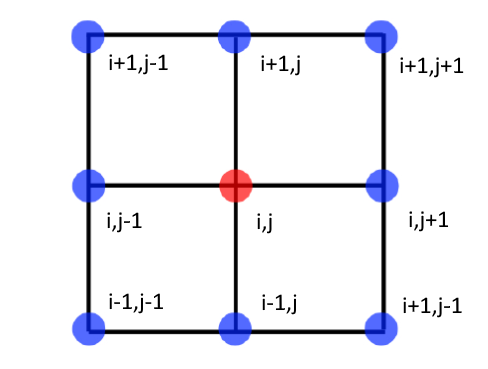
\includegraphics[width=0.4\linewidth]{images/9-point_stencil.png}
    \caption{Prikaz 9-točkovne matrice v dveh dimenzijah. Točka, ki jo posodabljamo, je obarvana rdeče, točke iz njene soseščine pa modro \cite{wiki:stencil-image}.}
    \label{fig:stencil}
\end{figure}

Matrice lahko predstavimo z matrikami, ki jih razširimo z ničlami, kjer ni koeficientov, da matriko zapolnimo.
Poleg računanja približkov odvodov lahko matrice uporabjamo tudi za druge aplikacije, na primer glajenje, ostrenje in iskanje robov na slikah. Zanimiva primera sta tudi Conwayeva igra življenja (angl. \textit{Conway's Game of Life}) in njegova posplošena oblika, Lenia \cite{lenia}.

V aplikacijah z vzorcem matrice v literaturi pogosto zasledimo pojem obroč (angl. \textit{halo}) \cite{anjum2022efficient}. To je obrobno območje na zunanji strani bloka ali mreže niti, ki vsebuje vrednosti, potrebne za izračun posodobljenih robnih vrednosti znotraj bloka oziroma mreže niti.

\section{Lenia}

Lenia sodi med celične avtomate (angl. \textit{cellular automaton}), v katerih je bila opažena pojavitev kompleksnih in avtonomnih vzorcev, podobnih pravim mikroorganizmom \cite{lenia}. V osnovi Lenia izhaja iz Conwayeve igre življenja in je dvodimenzionalni celični avtomat, ki deluje na podlagi stanja prostora-časa in generaliziranega lokalnega pravila.

V kontekstu računanja z matricami je Lenia lahko definirana kot primer aplikacije z vzorcem matrice z iterativno zanko (angl. \textit{iterative stencil loop}) \cite{7438873, enwiki:1334948319}, kjer v vsakem časovnem koraku simulacije posodobimo stanja vseh celic v avtomatu s pomočjo matrice.

Najprej definirajmo celične avtomate kot peterke \(\mathcal{A} = (\mathcal{L}, \mathcal{T}, \mathcal{S}, \mathcal{N}, \phi)\), kjer je:
\begin{itemize}
    \item \(\mathcal{L}\) mreža v \(D\) dimenzijah,
    \item \(\mathcal{T} = \{0, 1, 2, ..., T\}\), \(T \in \mathbb{Z}\) časovnica, ki nam pove, kolikokrat je potrebno posodobiti stanje mreže,
    \item \(\mathcal{S}\) množica stanj,
    \item \(\mathcal{N} \subset \mathcal{L}\) soseščina celice oziroma matrica in
    \item \(\phi : \mathcal{S}^\mathcal{N} \rightarrow \mathcal{S}\) lokalno pravilo, po katerem so definirani prehodi med stanji.
\end{itemize}
Definirati je potrebno tudi konfiguracijo oziroma skupek stanj v celotni mreži: \(\mathcal{A}^t : \mathcal{L} \rightarrow \mathcal{S}\) ob času \(t \in \mathcal{T}\). Pri tem \(\mathcal{A}^0\) predstavlja začetno konfiguracijo mreže.

Lenia, v primerjavi s Conwayevo igro življenja, ni omejena le na stanji 0 in 1, temveč ima lahko poljubno mnogo stanj: \(\mathcal{S} = \{0, 1, 2, ..., P\}\), \(P \in \mathbb{Z}\).
Njena matrica (\(\mathcal{N}\)) je prav tako razširjena iz Mooreove soseščine (9-točkovna dvodimenzionalna matrica \cite{enwiki:1333449780}, prikazana na sliki \ref{fig:stencil}) v poljubno velik diskretni krog \(\mathcal{N} = \{\mathbf{x} \in \mathcal{L} : \| \mathbf{x} \|_2 \le R\}\), \(R \in \mathbb{Z}\), kot prikazano na sliki \ref{fig:discrete-ball}.
Poleg teh razširitev Lenia normalizira stanja, soseščino in časovnico z recipročnimi vrednostmi \(\Delta x = 1 / R\), \(\Delta p = 1 / P\) in \(\Delta t = 1 / T\).
Od Conwayeve igre življenja se Lenia razlikuje tudi v lokalnem pravilu, ki je v diskretni Lenii definirano tako, da vsak časovni korak \(t\) v časovnici \(\mathcal{T}\) za vsako mrežno točko \(\mathbf{x}\) izračunamo konvolucijo z jedrom \(\mathbf{K} : \mathcal{N} \rightarrow \mathcal{S}\). Rezultat konvolucije je porazdelitev potenciala (angl. \textit{potential distribution}):
\begin{equation}
    \mathbf{U}^t (\mathbf{x}) = \mathbf{K} * \mathcal{A}^t (\mathbf{x}) = \sum_{\mathbf{n} \in \mathcal{N}} \mathbf{K}(\mathbf{n})\mathcal{A}^t(\mathbf{x} + \mathbf{n}) \Delta x^2
\end{equation}

\begin{figure}[H]
    \centering
    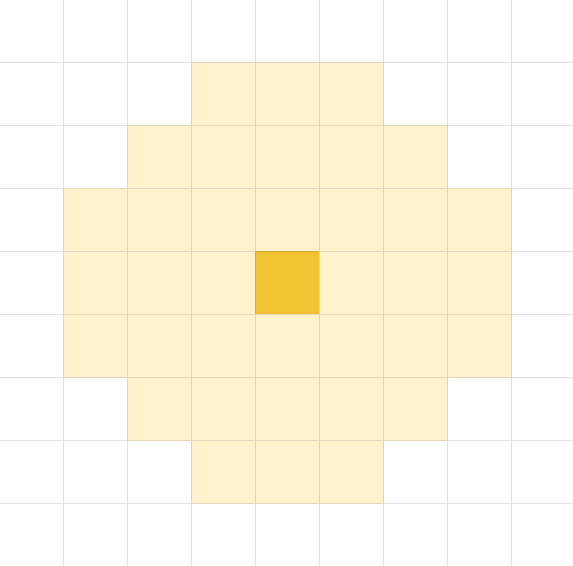
\includegraphics[width=0.4\linewidth]{images/stencil.png}
    \caption{Prikaz izgleda primera matrice za 2D Lenio.}
    \label{fig:discrete-ball}
\end{figure}

Operacijo konvolucije lahko izvedemo z matrico, ki predstavlja konvolucijsko jedro. Da izračunamo novo stanje celice, moramo na dobljeno porazdelitev potenciala aplicirati še rastno preslikavo (angl. \textit{growth mapping}) \(G : [0, 1] \rightarrow [0, 1]\). Rezultat je potencial rasti (angl. \textit{growth distribution}):
\begin{equation}
    \mathbf{G}^t (\mathbf{x}) = G(\mathbf{U}^t (\mathbf{x}))
\end{equation}

Porazdelitev rasti je potrebno pomnožiti z velikostjo časovnega koraka \(\Delta t\), to prišteti trenutni vrednosti celice in rezultat omejiti na interval \([0, 1]\):
\begin{equation}
    \mathbf{A}^{t + \Delta t} (\mathbf{x}) = [\mathbf{A}^t (\mathbf{x}) + \Delta t \mathbf{G}^t (\mathbf{x})]_{0}^{1}
\end{equation}

Jedro \(\mathbf{K}\) je sestavljeno iz jedrne (angl. \textit{kernel core}, \(K_C\)) in skeletne komponente (angl. \textit{kernel shell}, \(K_S\)). Obe sta preslikavi tipa \([0, 1] \rightarrow [0, 1]\).
Pri tem lahko jedrna komponenta zavzema obliko katerekoli unimodalne funkcije, ki zadostuje pogoju \(K_C(0) = K_C(1) = 0\). Izbiramo lahko med eksponentno, polinomsko, kvadratno ali katero drugo obliko.

Skeletna komponenta jedra kopira jedrno komponento v ekvidistančne koncentrične obroče glede na vektor \(\beta = (\beta_1, \beta_2, ..., \beta_B) \in [0, 1]^B\), ki definira faktorje, s katerimi skaliramo jedrno komponento. Skeletno komponento tudi normaliziramo, da velja \(\mathbf{K} * \mathbf{A} \in [0, 1]\).

Rastna preslikava lahko, podobno kot jedrna komponenta konvolucijskega jedra, zavzeva več oblik. Vsaka oblika mora biti unimodalna nemonotona funkcija s parametroma \(\mu, \sigma \in \mathbb{R}\), ki predstavljata center in širino rasti, pri čemer velja še \(G(\mu) = 1\).
Tudi v tem primeru lahko izbiramo med eksponentno, polinomsko, kvadratno ali katero drugo obliko funkcije.

Poleg opisane obstaja tudi zvezna različica Lenie \cite{lenia}, a se v tej nalogi osredotočamo na diskretno, saj jo lahko simuliramo numerično. Lenio je mogoče še dodatno razširiti, na primer povečati dimenzionalnost na tri dimenzije \cite{lenia_expanded}.

\section{Sorodna dela}

% Micikevicius (2009) — "3D Finite Difference Computation on GPUs using CUDA"
Paulius Micikevicius \cite{10.1145/1513895.1513905} je iskal optimizacijo aplikacij za računanje z metodo končnih razlik v okolju CUDA z minimiziranjem odvečnih pomnilniških dostopov.
Namesto predpomnjenja cele 3D kocke mrežnih točk je uporabil manjše 2D bloke niti, kjer so niti iterirale po kocki skozi posamezne ravnine točk v osi Z.
Pri tem so bili elementi trenutne ravnine predpomnjeni v skupnem pomnilniku, medtem ko so niti predpomnile elemente matrice v smeri osi Z v registrih, da so ustvarile drsajočo vrsto (ang. \textit{sliding queue}).
Ta zasnova računanja drastično zmanjša odvečna branja.

% High Performance Stencil Code Algorithms for GPGPUs
Avtorja Sch\"afer in Fey \cite{SCHAFER20112027} sta evalvirala aplikacije z vzorcem matrice na mikroarhitekturi Nvidia Fermi z uporabo Jacobijeve matrice pri meritvah zmogljivosti.
Evalvirani so bili trije algoritmi: naivno predpomnjenje cele soseščine matrice, iteriranje bloka niti 2D oblike skozi kocko mrežnih točk, kjer se predpomni le nekaj ploskev ter iteriranje po časovnem bloku dveh časovnih rezin, kjer ena nit izračuna dva časovna koraka namesto enega (angl. \textit{time/temporal tiling}). Avtorja slednjo tehniko imenujeta cevovodna valovna fronta (angl. \textit{pipelined wavefront}).
Ta pristop zmanjša potrebo po dostopih do globalnega pomnilnika in izboljša računsko učinkovitost.

% Anjum, Almasri, de Gonzalo in Hwu \cite{anjum2022efficient} so predstavili nov način učinkovitega računanja v aplikacijah na osnovi matric na GPE, imenovan SWiC (angl. \textit{scatter without write conflict}).
% Kot razlog za njegovo implementacijo so navedli slabosti dotedanjih pristopov. Prva slabost je osredotočenost na velike 3D matrice z vozlišči iz soseščine, ki so izključno na oseh (angl. \textit{axis-aligned grid points}).
% Za reševanje bolj kompleksnih problemov pogosto potrebujemo matrice z vozlišči, ki niso poravnana na osi, torej potrebujemo matrice z diagonalnimi vozlišči.
% Pri implementacijah, ki so upoštevale tudi točke izven osi, pa so kot slabost navedli 3D predpomnjenje, kjer je potrebno veliko deljenega pomnilnika, kar omejuje zasedenost GPE in s tem povzroči slabšo zmogljivost.
% Omenili so tudi pristop \textit{19P}, z dekompozicijo 55-točkovne matrice v manjše 19-točkovne ob večih obhodih.
% Pri tem so kot prednost navedli manjšo porabo deljenega pomnilnika, saj se predpomni 2D ploskev, kot slabosti pa so izpostavili večje število obhodov, slabšo aritmetično intenziteto in potrebo po takojšnjem pisanju razultatov v relativno počasen globalni pomnilnik.
% Navedene slabosti SWiC rešuje tako, da namesto vhodnih podatkov matrice v registre, shranjuje delne rezultate.
% Predpomni se le 2D ploskev in vsaka nit izračuna potrebne delne vsote, za katere je potrebna njena soležna predpomnjena vrednost, ter vsako shrani v svoj izhodni register. Izhodni registri so zasnovani v stilu cevovoda, kjer vsak register pripada svoji Z-ploskvi. Ko prejme register zadnjo potrebno delno vsoto, je končni rezultat napisan nazaj v globalni pomnilnik.
% Ta pristop zahteva le en obhod čez matrico, potrebno je relativno malo deljenega pomnilnika in ni pisnih konfliktov.

% High-Performance Code Generation for Stencil Computations on GPU Architectures
% Ker je implementirati različne ščepce GPE za matrice različnih tipov in velikosti zamudno ter otežuje vzdržljivost programske kode, se pojavi potreba po avtomatskemu generiranju ščepcev GPE za matrice.
% Ta problem naslavlja članek ``High-Performance Code Generation for Stencil Computations on GPU Architectures'' \cite{holewinski2012high}.
% Kot pogosto optimizacijsko tehniko v aplikacijah na osnovi matric so avtorji navedli časovno razvrščanje. Ta tehnika deluje na principu izračuna več časovnih korakov na podlagi istih podatkov, kar izboljša ponovno uporabo podatkov.
% Časovno razvrščanje tipično zahteva uporabo tehnike izvijanja zanke (angl. \textit{loop skewing}), ki prilagodi zaporedje iteracij, tako da so v skladu s podatkovnimi odvisnostmi. To uvede odvisnosti med časovnimi rezinami v prostorski domeni, zaradi česar je potrebno sinhronizirati časovne rezine in učinek paralelizma se zmanjša.
% Kot rešitev tega je omenjeno prekrivanje časovnih rezin (angl. \textit{overlapped tiling}), ki po eni strani prinese neodvisnost med rezinami, po drugi pa odvečno računanje ob robovih blokov.
% Iz praktičnih razlogov vzdržljivosti programske kode ščepcev, kjer bi sicer potrebovali ročno programirati ščepce za različne velikosti matrice, dimenzionalnosti in velikosti časovnih rezin, so avtorji predstavili ogrodje za avtomatsko generiranje kode. To prevajalniško usmerjeno ogrodje na podlagi visokonivojskega opisa matrice generira programsko kodo za ščepce GPE.

\chapter{Metodologija in orodja}
\label{metodologija}

\section{Implementacija}

V CUDA C/C++ smo implementirali Lenio z različnimi ščepci GPE.
Vsa programska koda je na voljo v repozitoriju na platformi GitHub \cite{repo}.

Relevantni parametri, po katerih ločujemo ščepce z različnimi strategijami sinhronizacije mreže, različnimi načini predpomnjenja ter polnjenja in naslavljanja skupnega pomnilnika, so:
\begin{itemize}
    \item dimenzija mreže (\(D\)),
    \item način sinhronizacije mreže (\(I\)),
    \item domena niti (\(P\)),
    \item način predpomnjenja (\(C\)) in
    \item strategija polnjenja skupnega pomnilnika (\(S\)).
\end{itemize}

Ostali pomembni parametri, ki določajo karakteristike posamezne simulacije, so:
\begin{itemize}
    \item velikost bloka niti (\(B\)),
    \item velikost mreže (\(W\)),
    \item število iteracij (\(T\)) in
    \item širina soseščine (\(R\)).
\end{itemize}

\subsection{Specifike implementacije Lenie}

Implementirali smo dvo- in trodimenzionalno različico Lenie.
Lenia dovoljuje različne oblike konvolucijskih jeder in različne metode preslikovanja rasti.
Za oboje smo izbrali eksponentni različici:
\begin{equation}
K_C(r) = \exp \left( \alpha - \frac{\alpha}{4r(1 - r)} \right),\quad\alpha = 4\quad\text{in}
\end{equation}

\begin{equation}
G(u; \mu, \sigma) = 2 \exp \left( - \frac{(u - \mu)^2}{2 \sigma^2} \right) - 1\quad.
\end{equation}

Za skeletno komponento konvolucijskega jedra smo izbrali enodimenzionalni vektor \(\beta\) z vrednostjo \(\beta_1 = 1\).
Ščepci GPE so implementirani tako, da imajo za mrežo točk ločena bralna in pisalna polja, kjer berejo iz bralnega, izračunajo novo stanje mreže in zapišejo rezultat v pisalno polje. Oba se nahajata v globalnem pomnilniku.
Začetno stanje mreže, \(\mathcal{A}^0\), smo inicializirali z naključnimi števili iz intervala \([0, 1]\).
Zaradi lažjega preverjanja pravilnosti delovanja smo vedno uporabili enako seme za generator psevdonaključnih števil.
Delali smo le s števili v plavajoči vejici z enojno natančnostjo (32 bitov). Z natačnostjo le-teh je implicitno implementirana diskretizacija stanj (\(\Delta p\)).

\subsection{Način sinhronizacije mreže}

Pri simulaciji Lenie, ki traja \(T\) iteracij, moramo v vsaki iteraciji posodobiti stanje vseh celic v mreži. Pri tem lahko izbiramo med dvema načinoma sinhronizacije mreže niti:
\begin{enumerate}[label=(\alph*)]
    \item na gostitelju (CPE) iteriramo v zanki na intervalu od 1 do \(T\) in v vsaki iteraciji kličemo ščepec CUDA, ki bo posodobil stanja celic v mreži.
    \item Na gostitelju le enkrat sprožimo ščepec, zanko premaknemo znotraj njega in tam izvajamo izračune novih stanj ter mrežo po vsaki iteraciji sinhroniziramo.
\end{enumerate}

Slednja možnost je relevantna, ker se z njo znebimo režije pri vsakokratnem klicu ščepca.
Za sinhronizacijo na GPE nam CUDA za reševanje tega problema ponuja funkcionalnost sodelovalnih skupin (angl. \textit{cooperative groups}), ki omogoča postavitev prepreke za vse niti v mreži.
Posledica tega je, da mora biti mreža dovolj majhna, da se lahko vsi bloki niti hkrati izvajajo na GPE.
Pri načinu sinhronizacije mreže na GPE je za pravilno delovanje potrebno po vsaki iteraciji še zamenjati vlogi bralnega in pisalnega polja.
To storimo z zamenjavo kazalcev na omenjene kose pomnilnika.

V nalogi sta implementirana oba načina. V rezultatih ju ločujemo glede na parameter \(I\):
\begin{displaymath}
    I = \begin{cases}
        0, & \text{sinhronizacija mreže preko CPE}    \\
        1, & \text{sinhronizacija mreže preko GPE}
    \end{cases}\quad.
\end{displaymath}

\subsection{Širina soseščine}

Širina soseščine (\(R\)) določa velikost matrice Lenie z izrazom \((2R + 1) ^ D\). Vsi ščepci podpirajo dinamično veliko soseščino.

\subsection{Velikost bloka in mreže}

Bloki niti so velikosti \(B^D\), mreže pa \(W^D\).
Parameter \(W\) predstavlja velikost mreže v celicah v eni dimenziji in je vedno oblike \(2^N, N \in \mathbb{N}\).
Razlog za to je v strategiji obravnave roba mreže, kjer smo izbrali ovijanje okoli nje.
To storimo tako, da želenemu indeksu celice prištejemo velikost mreže v isti dimenziji ter nadalje izvedemo operacijo modulo z velikostjo mreže v isti dimenziji. Primer:
\verb|x = (x + W) % W;|.
Težava tega pristopa je, da so operacije modulo na GPE relativno počasne v primerjavi z operacijami, kot sta seštevanje in odštevanje.
To lahko pohitrimo tako, da zamenjamo modulo z bitno konjunkcijo z za eno zmanjšanim operandom.
To lahko storimo le, če je operand potenca števila dve, kar privede do ekvivalentne operacije:
\verb|x = (x + W) & (W - 1);|.

Prav tako, kot pri načinu sinhronizacije mreže, velja omeniti tudi, da smo omejeni pri izbiri velikosti blokov niti.
Večji bloki niti pomenijo manjše število blokov, ki se lahko hkrati izvajajo na GPE in na računskih enotah, ko uporabljamo skupni pomnilnik. Velikost slednjega je omejena na računsko enoto, kar pomeni da si morajo bloki, ki se izvajajo na isti računski enoti, skupni pomnilnik deliti.
Poleg tega omejitev predstavlja tudi število registrov, ki je tudi omejeno in si jih morajo bloki znotraj računske enote deliti.

\subsection{Domena niti}

V aplikacijah z vzorcem matrice predpostavimo, da bo vsaka nit v bloku niti izračunala posodobljeno stanje le svoje soležne celice v mreži.
Alternativa temu je, da vsaka nit posodobi stanje večih celic. Tako lahko na primer zmanjšamo velikost bloka niti za eno dimenzijo iz \(B^D\) na \(B^{D-1}\).
V taki situaciji mora vsaka nit v zanki iterirati čez \(B\) ravnin in v vsaki posodobiti stanje ene celice, kot je predstavil Micikevicius \cite{10.1145/1513895.1513905}.
Tu pride do ločitve na bloke niti in bloke celic, ki so tako po velikosti večje ali enake blokom niti.
Za lažje ločevanje bomo v nadaljevanju za bloke celic v primeru 3D mreže uporabljali izraz kocka, v primeru 2D mrež pa izraz kvadrat.
V praksi v dvodimenzionalni mreži iteriramo po vrsticah kvadrata v dimenziji Y, v 3D mreži pa po ravninah v dimenziji Z ter na vsakem koraku z matrico izračunamo novo stanje celice.

Tak sistem je predvsem uporaben za zmanjšanje velikosti bloka in izboljšanje zasedenosti GPE, ko imamo opravka z velikimi bloki niti, ki lahko porabijo veliko skupnega pomnilnika ali veliko registrov.

Pri prvem načinu je torej domena niti ena celica, v drugem pa en stolpec znotraj kocke oziroma kvadrata. V diplomski nalogi sta implementirana oba načina, v rezultatih ju ločimo s parametrom \(P\):
\begin{displaymath}
    P = \begin{cases}
        0, & \text{domena niti je celica}    \\
        1, & \text{domena niti je stolpec}
    \end{cases}\quad.
\end{displaymath}

\subsection{Način predpomnjenja}

Za pohitritev izvajanj ščepcev uporabimo skupni pomnilnik.
Poleg različice brez predpomnjenja sta implementirana dva načina uporabe skupnega pomnilnika, ki ju v rezulatih naloge ločujemo glede na parameter \(C\):
\begin{displaymath}
    C = \begin{cases}
        0, & \text{brez predpomnjenja} \\
        1, & \text{predpomnjenje kocke oziroma kvadrata in obroča okoli} \\
        2, & \text{predpomnjenje bloka niti in obroča}
    \end{cases}\quad.
\end{displaymath}

\subsubsection{Predpomnjenje kocke oziroma kvadrata in obroča}

V prvem načinu predpomnimo celotno kocko oziroma kvadrat in obroč okoli njega.
Širina obroča je enaka širini soseščine matrice, da imamo lahko v skupnem pomnilniku na voljo vse podatke za posodobitev stanj vseh celic znotraj kocke oziroma kvadrata.
V tem načinu najprej prenesemo potrebne podatke v skupni pomnilnik in nato izračunamo novo stanje celice z matrico.

\subsubsection{Predpomnjenje mreže, ki jo pokrivata blok niti in njegov obroč}

Drugi način zahteva predpomnjenje dela mreže, ki jo pokriva blok niti ter obroča okoli njega.
Širina obroča je enaka kot pri prvem načinu. Ko je domena niti ena celica, sta blok niti in kocka oziroma kvadrat niti po velikosti enaka, zato je ta način uporabljen le v primeru, ko je domena niti stolpec.
Ker imamo pri domeni stolpca v predpomnilniku prostora le za blok niti in obroč, moramo za vsako vrstico (2D) oziroma ploskev (3D) najprej zamakniti vrednosti v skupnem pomnilniku za eno vrstico navpično navzgor, da lahko spodaj ustvarimo prostor za prenos nove vrstice oziroma ploskve iz globalnega v skupni pomnilnik. Za tak pristop je pred izvedbo zanke potreben še predprenos prvega bloka niti in obroča v predpomnilnik.
Posledično lahko zmanjšamo porabo skupnega pomnilnika v primerjavi s prvim načinom predpomnjenja.

\subsection{Strategija polnjenja skupnega pomnilnika}

Skupni pomnilnik lahko polnimo na več načinov. Če bi bila velikost skupnega pomnilnika enaka velikosti bloka niti, bi lahko vsaka nit prenesla po eno soležno vrednost iz globalnega v skupni pomnilnik. Naša implementacija je taka, da skupni pomnilnik vedno vsebuje tudi obroč, katerega velikost je odvisna od širine soseščine matrice, da skupni pomnilnik vedno vsebuje več celic kot je niti v bloku. To pomeni, da morajo nekatere niti opraviti več dela kot druge.

Vsaka nit v bloku v zanki prenaša vrednosti celic, dokler so celice še na voljo.
V primeru, ko je domena niti ena celica, bi \(B^D\) niti v bloku preneslo \((2R + B)^D\) celic.
V drugem primeru, ko je domena niti en stolpec, bi \(B^{D - 1}\) niti v bloku preneslo \((2R + B)^D\) celic, ko predpomnimo kocko oz. kvadrat in obroč okoli njega, oziroma \((2R + B)^{D - 1} \times (2R + 1)\) celic, ko predpomnimo le blok niti z obročem.
Posledično z naraščanjem velikosti širine soseščine matrice in manjšanjem bloka niti narašča količina celic, ki jih mora vsaka nit prenesti iz globalnega v skupni pomnilnik, saj večji delež volumna skupnega pomnilnika predstavlja obroč.

Implementirali smo tri različne mehanizme za polnjenje skupnega pomnilnika, ločujemo jih s parametrom \(S\):
\begin{displaymath}
    S = \begin{cases}
        1, & \text{strategija 1} \\
        2, & \text{strategija 2} \\
        3, & \text{strategija 3} \\
    \end{cases}\quad.
\end{displaymath}

\subsubsection{Strategija 1}

Prva strategija (\(S=1\)) je implementirana kot enojna zanka \texttt{while} po principu vrstične (angl. \textit{row major}) krožne zanke (angl. \textit{round robin}).
Vsaka nit v skupni pomnilnik skopira soležno vrednost iz globalnega pomnilnika in se nato premakne za \(B^D\) celic naprej po območju, ki ga je potrebno prenesti v skupni pomnilnik.
Na sliki \ref{fig:S1} je videti logika kroženja niti po vrsticah, kjer 16 niti iz bloka velikosti \(4^2\) (temnejše območje) polni predpomnilnik velikosti \(6^2\), z obročem, širokim eno celico (svetlejše območje).

\begin{figure}[H]
    \centering
    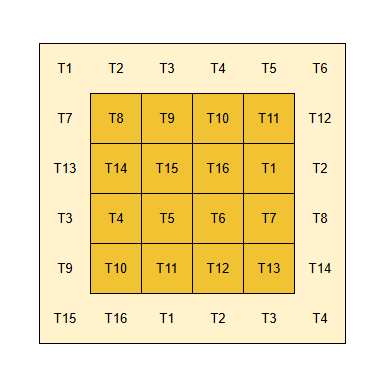
\includegraphics[width=0.6\linewidth]{images/S1.png}
    \caption{Prikaz polnjenja predpomnilnika s krožno zanko \texttt{while} po vrsticah. S temnejšo barvo je označeno soležno območje bloka niti, s svetlejšo pa obroč okoli njega.}
    \label{fig:S1}
\end{figure}

Iz izseka kode \ref{lst:s1} je razvidno, da potrebujemo enodimenzionalni indeks celice pretvoriti v posamezne komponente po dimenzijah. Pri tem moramo za vsako celico opraviti po dve operaciji deljenja in dve operacije modulo v 3D mreži oziroma po eno v 2D mreži. Obe vrsti operacij sta relativno počasni za izvajanje na GPE.

\begin{lstlisting}[language=c++, caption=Izsek kode s primerom mehanizma za predpomnjenje kocke v 3D mreži z enojno zanko \texttt{while}., basicstyle=\scriptsize\ttfamily, frame=single, label=lst:s1]
dim3 cache_dims(
    blockDim.x + 2 * R,
    blockDim.x + 2 * R,
    blockDim.x + 2 * R
);
int cache_volume = cache_dims.x * cache_dims.y * cache_dims.z;
int curr_index_1D = (
    blockDim.x * blockDim.y * threadIdx.z
    + blockDim.x * threadIdx.y
    + threadIdx.x
);
int cache_start_x = blockIdx.x * blockDim.x - R;
int cache_start_y = blockIdx.y * blockDim.y - R;
int cache_start_z = blockIdx.z * blockDim.z - R;
while (curr_index_1D < cache_volume) {
    remainder = curr_index_1D % (cache_dims.x * cache_dims.y);

    curr_cell_z = cache_start_z + curr_index_1D / (
        cache_dims.x * cache_dims.y
    );
    curr_cell_y = cache_start_y + remainder / cache_dims.x;
    curr_cell_x = cache_start_x + remainder % cache_dims.x;

    // Ovijanje okoli mreze
    curr_cell_z = (curr_cell_z + W) & (W - 1);
    curr_cell_y = (curr_cell_y + W) & (W - 1);
    curr_cell_x = (curr_cell_x + W) & (W - 1);

    cache[curr_index_1D] = world[
        W * W * curr_cell_z
        + W * curr_cell_y
        + curr_cell_x
    ];

    // Skoci k naslednji celici
    curr_index_1D += blockDim.x * blockDim.y * blockDim.z;
}
\end{lstlisting}

\subsubsection{Strategija 2}

Druga strategija (\(S=2\)) je implementirana kot gnezdene zanke \texttt{for} v vrstični logiki, da lahko izkoristimo prostorsko lokalnost podatkov z združenimi branji (angl. \textit{coalesced reads}).
Od prve strategije se razlikuje še v tem, da se z zankami \texttt{for} izognemo operacijam modulo in operacijam deljenja (\ref{lst:s2}), ki smo jih potrebovali za izračun globalnih indeksov celic.
Na sliki \ref{fig:S2} je razvidna logika polnjenja predpomnilnika po vrsticah, kjer 16 niti iz bloka velikosti \(4^2\) (temnejše območje) polni predpomnilnik velikosti \(6^2\), z obročem, širokim eno celico (svetlejše območje).
Razvidno je, da nekatere niti ne opravljajo nobenega dela.

\begin{figure}[H]
    \centering
    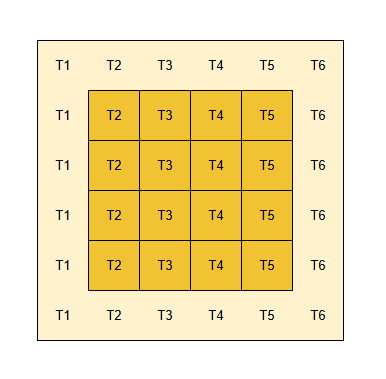
\includegraphics[width=0.6\linewidth]{images/S2.png}
    \caption{Prikaz polnjenja predpomnilnika z gnezdenimi zankami \texttt{for} v vrstični logiki. S temnejšo barvo je označeno soležno območje bloka niti, s svetlejšo pa obroč okoli njega.}
    \label{fig:S2}
\end{figure}

\begin{lstlisting}[language=c++, caption=Izsek kode z mehanizmom za predpomnjenje kocke v 3D mreži z gnezdenimi zankami \texttt{for} v vrstični logiki., basicstyle=\scriptsize\ttfamily, frame=single, label=lst:s2]
dim3 cache_dims(
    blockDim.x + 2 * R,
    blockDim.x + 2 * R,
    blockDim.x + 2 * R
);
for (int z = threadIdx.z; z < cache_dims.z; z += blockDim.z) {
    curr_cell_z = blockIdx.z * blockDim.z - R + z;
    // Ovijanje okoli mreze
    curr_cell_z = (curr_cell_z + W) & (W - 1);

    for (
        int y = threadIdx.y; y < cache_dims.y; y += blockDim.y
    ) {
        curr_cell_y = blockIdx.y * blockDim.y - R + y;
        // Ovijanje okoli mreze
        curr_cell_y = (curr_cell_y + W) & (W - 1);

        for (
            int x = threadIdx.x; x < cache_dims.x; x += blockDim.x
        ) {
            curr_cell_x = blockIdx.x * blockDim.x - R + x;
            // Ovijanje okoli mreze
            curr_cell_x = (curr_cell_x + W) & (W - 1);

            cache[
                z * cache_dims.x * cache_dims.y
                + y * cache_dims.x
                + x
            ] = world[
                W * W * curr_cell_z
                + W * curr_cell_y
                + curr_cell_x
            ];
        }
    }
}
\end{lstlisting}

\subsubsection{Strategija 3}

Zadnja obravnavana strategija (\(S=3\)) je v obliki gnezdenih zank \texttt{for}, a v stolpični (angl. \textit{column major}) logiki, kar implicira potencialno počasnejše delovanje zaradi nezdruženih branj.
Tako kot v drugi strategiji se v tretji prav tako izognemo operacijam modulo in operacijam deljenja.
Ker tokrat polnimo skupni pomnilnik stolpično (\ref{lst:s3}), moramo iz slednjega tako tudi brati.
Na sliki \ref{fig:S3} je razvidna logika polnjenja predpomnilnika po stopcih, kjer 16 niti iz bloka velikosti \(4^2\) (temnejše območje) polni predpomnilnik velikosti \(6^2\), z obročem, širokim eno celico (svetlejše območje).
Tudi v tem primeru je razvidno, da nekatere niti ne opravljajo nobenega dela.

\begin{figure}[H]
    \centering
    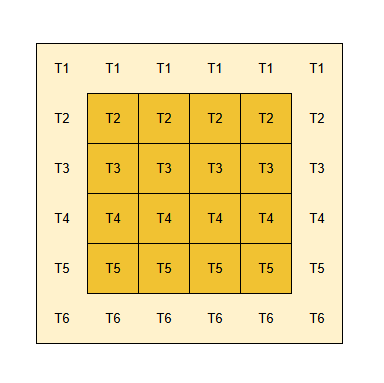
\includegraphics[width=0.6\linewidth]{images/S3.png}
    \caption{Prikaz polnjenja predpomnilnika z gnezdenimi zankami \texttt{for} v stolpični logiki. S temnejšo barvo je označeno soležno območje bloka niti, s svetlejšo pa obroč okoli njega.}
    \label{fig:S3}
\end{figure}

\begin{lstlisting}[language=c++, caption=Izsek kode s primerom mehanizma za predpomnjenje kocke v 3D mreži z gnezdenimi zankami \texttt{for} v stolpični logiki., basicstyle=\scriptsize\ttfamily, frame=single, label=lst:s3]
dim3 cache_dims(
    blockDim.x + 2 * R,
    blockDim.x + 2 * R,
    blockDim.x + 2 * R
);
for (int x = threadIdx.x; x < cache_dims.x; x += blockDim.x) {
    curr_cell_x = blockIdx.x * blockDim.x - R + x;
    // Ovijanje okoli mreze
    curr_cell_x = (curr_cell_x + W) & (W - 1);

    for (
        int y = threadIdx.y; y < cache_dims.y; y += blockDim.y
    ) {
        curr_cell_y = blockIdx.y * blockDim.y - R + y;
        // Ovijanje okoli mreze
        curr_cell_y = (curr_cell_y + W) & (W - 1);

        for (
            int z = threadIdx.z; z < cache_dims.z; z += blockDim.z
        ) {
            curr_cell_z = blockIdx.z * blockDim.z - R + z;
            // Ovijanje okoli mreze
            curr_cell_z = (curr_cell_z + W) & (W - 1);

            cache[
                cache_dims.z * cache_dims.y * x
                + y * cache_dims.z
                + z
            ] = world[
                W * W * curr_cell_z
                + W * curr_cell_y
                + curr_cell_x
            ];
        }
    }
}
\end{lstlisting}

\subsection{Število iteracij in meritve časov izvajanj}

Število iteracij (\(T\)) se nanaša na dolžino simulacije Lenie.
Pove nam, kolikokrat se posodobi stanje mreže.
Pri meritvah smo iz praktičnih razlogov pri različnih velikostih mreže uporabili različne vrednosti števila iteracij simulacije.
Ker bi pri trodimenzionalni mreži simulacija trajala precej dlje kot po ostalih parametrih analogna simulacija v dvodimenzinalni mreži, smo pri 3D različicah zmanjšali število iteracij.
Po drugi strani je bilo potrebno število slednjih povečati pri različicah, kjer mrežo sinhroniziramo preko GPE, zaradi omejitev pri velikostih mreže.
Posledično je čas izvajanja simulacije nezadostna mera.
Bolj primeren je čas, porabljen za posamezno iteracijo simulacije Lenie:
\begin{equation}
    \text{čas/iter.} = \frac{\text{povprečen izmerjen čas simulacije}}{T}\quad.
\end{equation}

\section{Izvajanje meritev}

Cilj je izmeriti čase izvajanj simulacij Lenie za vse smiselne konfiguracije parametrov, izračunati povprečne čase izvajanj in jih primerjati.

Za preverjanje pravilnosti simulacij Lenie smo implementirali različico, ki se v celoti izvaja na CPE, brez paralelizma, ter rezultate primerjali z rezultati simulacij vseh relevantnih kombinacij parametrov.

Bolj kot primerjava z različico brez paralelizma nas je zanimala primerjava zmogljivosti simulacij s tistimi brez predpomnenja in z domeno niti enako celici. Zato smo enačbo za pohitritev nekoliko prilagodili:
\begin{equation}
    S(n, p) = \frac{t_p(n, p; C=0, P=0)}{t_p(n, p)}\quad.
\end{equation}
Simulacij različnih dimenzionalnosti in različnega načina sinhronizacije mreže med sabo nismo primerjali.

Vsako konfiguracijo simulacije smo v meritvah izvajanj pognali po desetkrat in izračunali povprečen čas izvajanja na iteracijo, standardni odklon meritev ter pohitritev.

Programska koda je bila prevedena s prevajalnikom \textit{nvcc} tako, kot je prikazano v izseku kode \ref{lst:makefile}.

\begin{lstlisting}[language=sh, caption=Izsek kode \textit{Makefile} za prevajanje aplikacije., basicstyle=\scriptsize\ttfamily, frame=single, label=lst:makefile]
nvcc -Wno-deprecated-gpu-targets \
    -Xcompiler -fopenmp \
    -dc -g -G \
    -I $(HEADERS_COMMON) \
    -I $(HEADERS_KERNELS_2D) \
    -I $(HEADERS_KERNELS_3D) \
    -odir build \
    $(ALL_SOURCES)

nvcc -Wno-deprecated-gpu-targets \
    -lgomp \
    -g -G \
    -o lenia \
    $(shell ls build/*.o)
\end{lstlisting}

Omenjene GPE imajo omejitev 48 kB skupnega pomnilnika na blok niti, kar pomeni, da lahko pri predpomnjenju relativno hitro pridemo do največje možne soseščine, še posebej v 3D simulacijah.

Velikosti bloka niti, ki smo jih vključili simulacije, so bile pri 2D mreži \(8^2\) in \(16^2\), medtem ko so bile pri 3D mreži \(4^3\) in \(8^3\).
Širine soseščin, ki smo jih vključili v meritve, so bile na intervalu \([1, 14]\).
Kjer omejitev skupnega pomnilnika ni dopuščala večjih soseščin, smo se omejili na največje še možne soseščine, ki so bile na intervalu \([7, 10]\), odvisno od velikosti bloka in načina predpomnjenja.
Velikosti mrež, ki smo jih uporabili, so se razlikovale glede na dimenzionalnost in način sinhronizacije mrež.
Kjer smo mrežo sinhronizirali preko CPE, smo za 2D mrežo uporabili velikost \(2024^2\) celic, za 3D pa \(128^3\) celic.
Pri meritvah simulacij s sinhronizacijo mreže preko GPE smo bili omejeni zaradi uporabe sodelovalnih skupin.
V meritvah 2D simulacij smo pri blokih \(8^2\) bili omejeni na mrežo velikosti \(128^2\) celic, pri blokih \(16^2\) pa na \(256^2\) celic.
Kljub temu smo pri slednjih za lažjo primerjavo z manjšimi bloki tudi uporabili mrežo velikosti \(128^2\) celic.
3D simulacje so prinesle še večje omejitve.
Pri blokih \(4^3\) smo morali mrežo zmanjšati na \(32^3\) celic.
Enaka omejitev je bila za večje bloke \(8^3\), razen v primeru, ko smo za domeno niti izbrali cel stolpec, ko je omejitev znašala \(64^3\) celic.
Zaradi lažjih primerjav smo pri slednji konfiguraciji prav tako ostali na enaki velikoti mreže kot pri manjših blokih.

Da smo maksimizirali potencial in poiskali omejitev, smo z API klicem funkcije \texttt{cudaOccupancyMaxActiveBlocksPerMultiprocessor} izračuli, koliko blokov niti željene velikosti se lahko hkrati izvaja na eni računski enoti. Pri tem se upošteva še željena velikost skupnega pomnilnika in ščepceva poraba registrov.

\subsection{Strojna oprema}

Meritve smo izvajali na Arnesovi gruči, na vozliščih, ki imajo na voljo Nvidia H100 GPE mikroarhitekture Grace Hopper.
Slednje imajo 132 računskih enot, kjer lahko vsaka hkrati izvaja največ 2048 niti.
Vsaka računska enota ima na voljo največ 65536 registrov ter 228 kB skupnega pomnilnika.
Poleg tega ima omejitev 48 kB skupnega pomnilnika na blok niti.

% \section{Programska oprema}

% Za namene primerjave različnih metod računanja šablon bodo le-te tudi implementirane, in sicer v programskem jeziku CUDA C++. Programsko kodo bom razvijal lokalno, na operacijskem sistemu Windows 11 z nameščenim okoljem za razvijanje Visual Studio Code z vtičnikom Nvidia Nsight. Okolje bo povezano na virtualni stroj WSL Ubuntu. Poleg tega se bodo potrebovali tudi gonilniki CUDA za GPE.

% Testiranje programske kode bo potekalo na računski gruči Arnes, saj ponujajo zmogljive GPGPE. Upravljanje takšne gruče poteka preko sistema Slurm.

% software: VS Code, WSL Ubuntu, Win 11 Education, SLURM, Python for results analysis (Polars and Matplotlib), CUDA toolkit 12.8(?)

\chapter{Rezultati in razprava}
\label{rezultati}

V tem poglavju bodo prikazani časi izvajanj vseh konfiguracij parametrov v obliki tabel in stolpičnih diagramov.
Rezultate smo razdelili glede na dimenzionalnost in način iteracije simulacije.
Za lažje označevanje smo za ločevanje med različnimi konfiguracijami uporabili pripadajoče parametre.
Vključene tabele s pohitritvami prikazujejo širino soseščine 7.
Na grafih, kjer so prikazani časi izvajanja na iteracijo simulacije za konfiguracije z domeno niti enako stolpcu, smo za lažjo primerjavo vključili tudi osnovno konfiguracijo brez predpomnjenja in z domeno niti enako celici.

\section{2D}

Za dvodimenzionalno mrežo smo izbrali velikosti stranic blokov niti \(B=8\) in \(B=16\).
Bloki so tako imeli po \(8^2\) oziroma \(16^2\) celic pri domeni niti ene celice (\(P=0\)) in \(8^1\) ter \(16^1\) celic v primeru, ko je domena niti stolpec (\(P=1\)).

\subsection{Sinhronizacija mreže preko CPE}

Pri sinhronizaciji mreže preko CPE (\(I=0\)) smo za njeno velikost izbrali \(W = 2048\), kar je skupaj \(2048^2\) celic.
Za bloke pri \(B=8\) je bil največji izmerjeni standardni odklon meritev 0,174 ms, pri \(B=16\) pa 0,187 ms.

% 2D I0 P0
Iz stolpičnih diagramov \ref{fig:2D_I0_P0_B8} in \ref{fig:2D_I0_P0_B16} je razvidno, da so različice s predpomnjenjem nekoliko hitrejše od tistih brez predpomnjenja, ko je domena niti ena celica.
Opaziti je načeloma rahlo hitrejše čase izvajanj za strategijo 2 v primerjavi s strategijo 1, kar je smiselno, če upoštevamo, da druga strategija ne vsebuje relativno počasnih operacij deljenja in modula.
V nasprotju s pričakovanji je tretja strategija hitrejša od predhodnjih.
Navedena strategija namreč implementira stolpično logiko naslavljanja elementov v skupnem pomnilniku, ki naj bi po pričakovanjih negativno vplivala na hitrost.
Za ta primer nismo našli razloga za njegove čase izvajanj in bi zato bilo potrebno dodatno raziskovanje.

Velja tudi omeniti, da so pri manjših soseščinah razlike med strategijami polnjenja predpomnilnika, tudi v primerjavi s strategijo brez predpomnjenja zelo majhne oziroma tudi zanemarljive. Ko se soseščina veča, pa pride do bolj pomembnih razlik. Podoben trend obstaja tudi pri vseh ostalih prikazih rezultatov simulacij.

Poleg tega je razvidno tudi, da pri konfiguracijah iz diagramov \ref{fig:2D_I0_P0_B8} in \ref{fig:2D_I0_P0_B16} velikost bloka ni vplivala na čase izvajanj, ki so se pri najveji soseščini R=14 gibali nad 22 ms na iteracijo za različice brez predpomnjenja in okoli 19 ms za vse različice s predpomnjenjem.

Iz vseh diagramov, tudi v nadaljevanju, je razvidna eksponentna rast časov izvajanja na iteracijo simulacije ob enakomernem naraščanju širine soseščine matrice.

V tabelah \ref{tab:2D_I0_B8} in \ref{tab:2D_I0_B16} so podane pohitritve, ki so izračunane glede na konfiguracije iste dimenzije in metode sinhronizacije mreže, a brez predpomnenja in z domeno niti enako celici.
Iz tabel je razvidno, da so pohitritve pri tej soseščini pri P=0 okoli 1,1- do 1,17-kratne, glede na strategijo polnjenja predpomnilnika. Podobno velja za večje soseščine.
\raggedbottom

\begin{figure}[H]
    \centering
    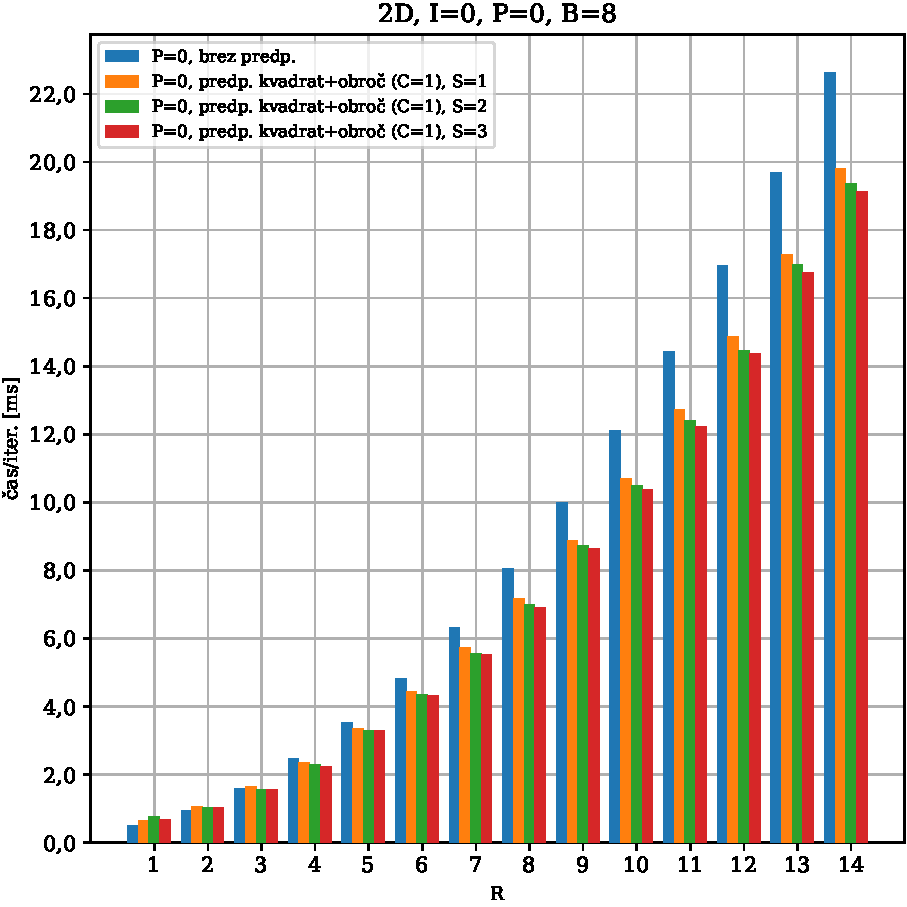
\includegraphics[width=0.7\linewidth]{images/2D_I0_P0_B8.pdf}
    \caption{Diagram časov izvajanj pri različnih soseščinah in strategijah polnjenja predpomnilnika. Velikost bloka: \(8^2\), domena niti: celica, sinhronizacija mreže: CPE.}
    \label{fig:2D_I0_P0_B8}
\end{figure}

\begin{figure}[H]
    \centering
    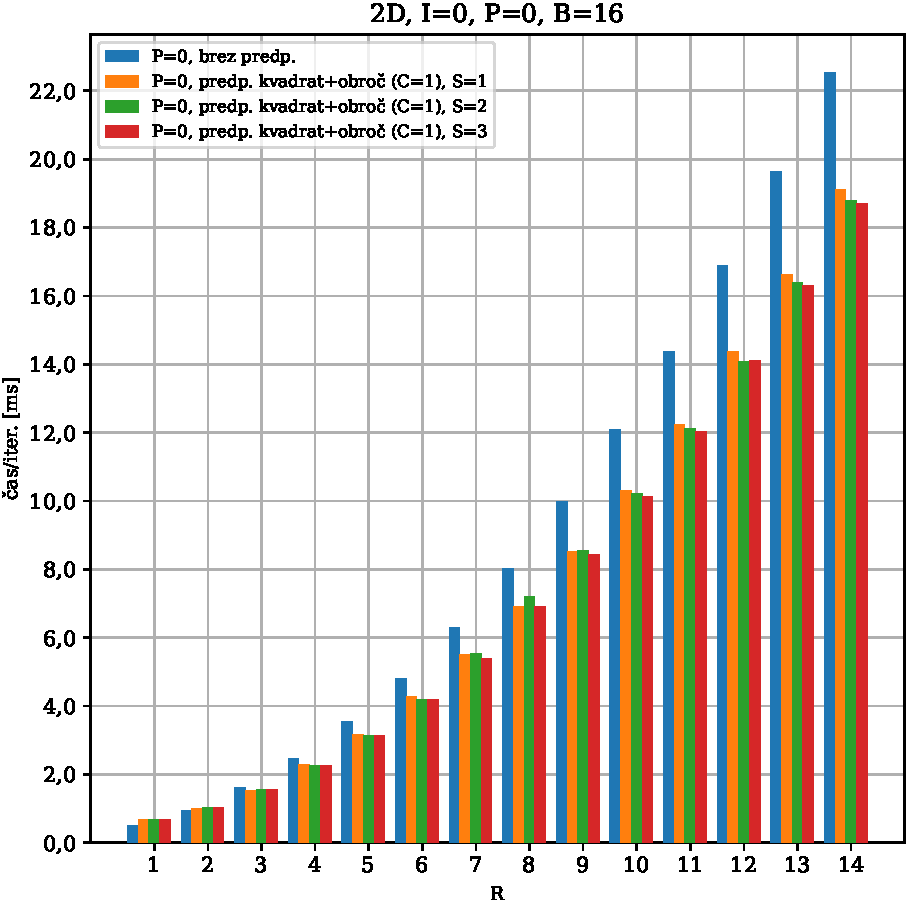
\includegraphics[width=0.7\linewidth]{images/2D_I0_P0_B16.pdf}
    \caption{Diagram časov izvajanj pri različnih soseščinah in strategijah polnjenja predpomnilnika. Velikost bloka: \(16^2\), domena niti: celica, sinhronizacija mreže: CPE.}
    \label{fig:2D_I0_P0_B16}
\end{figure}

% 2D I0 P1
Razlike se opaže pri primeru P=1, ko je domena niti stolpec.
S tem se blok niti zmanjša za eno dimenzijo na \(8^1\), oziroma \(16^1\).
Iz diagrama \ref{fig:2D_I0_P1_B8} je razvidno, da časi izvajanj na iteracijo simulacije skokovito narastejo, namesto, da bi padli.
Pri širini soseščine 14 je tako čas izvajanja na iteracijo pri P=1 in brez predpomnjenja pibližno 104 ms, torej približno petkrat večji, kot pri P=0.
Pohitritev je namreč 0,22-kratna.
Podobne upočasnitve veljajo tudi za različice s predpomnjenjem.

Kjer predpomnimo celoten kvadrat in obroč, je upočasnitev okoli 4-kratna, s časi izvajanj na iteracijo od 87 do 90 ms pri največji soseščini.
Prva strategija je tudi v tej konfiguraciji najpočasnejša, čeprav le minimalno.
Najhitrejša je tretja strategija.

Enako ne moremo trditi za konfiguracije, kjer predpomnimo blok niti in obroč (C=2).
Tu se časi izvajanj pri največji soseščini gibljejo okoli 101 ms.
Druga strategija (gnezdena zanka \texttt{for}, vrstična logika) je najpočasnejša, prva (vrstična krožna zanka \texttt{while}) je rahlo hitrejša in tretja strategija (gnezdena zanka \texttt{for}, stolpična logika) je najhitrejša.

Ob povečavi bloka iz \(8^1\) na \(16^1\) je iz diagramu \ref{fig:2D_I0_P1_B16} mogoče prepoznati skoraj 2-krat manjše upočasnitve.
Poleg tega je med strategijami polnjenja predpomnilnika opazna tudi nekonsistentnost pri hitrostih izvajanja na iteracijo.
Pri večini soseščin se razmerja hitrosti skladajo s tistimi iz diagrama \ref{fig:2D_I0_P1_B8}, razen pri dveh največjih soseščinah.
Pri slednjih so strategije polnjenja predpomnilnika kvadrata in obroča približno tako hitre kot strategija brez predpomnjenja z domeno niti stolpca in počasnejše od strategij s predpomnjenjem bloka niti in obroča.

Pomembno je izpostaviti, da je pri konfiguracijah z domeno niti enaki stolpcu blok vedno manjši od enega snopa.
Pri takšnih konfiguracijah se bo zgodilo, da vsak blok niti zasedel svoj snop, pri tem bodo pa v vsakem snopu nekatere niti ostale neuporabljene.
Z zmanjšanjem paralelizma pade tudi zmogljivost aplikacije.
Posledica tega so upočasnitve, ki se odražajo na diagramih in v tabelah.
Dvakrat manjše upočasnitve pri blokih \(16^1\) kot pri \(8^1\) sovpadajo tudi s tem, da je prvi blok dvakrat večji od drugega, kar pomeni dvakrat manj neuporabljenih niti znotraj snopa.

\begin{figure}[H]
    \centering
    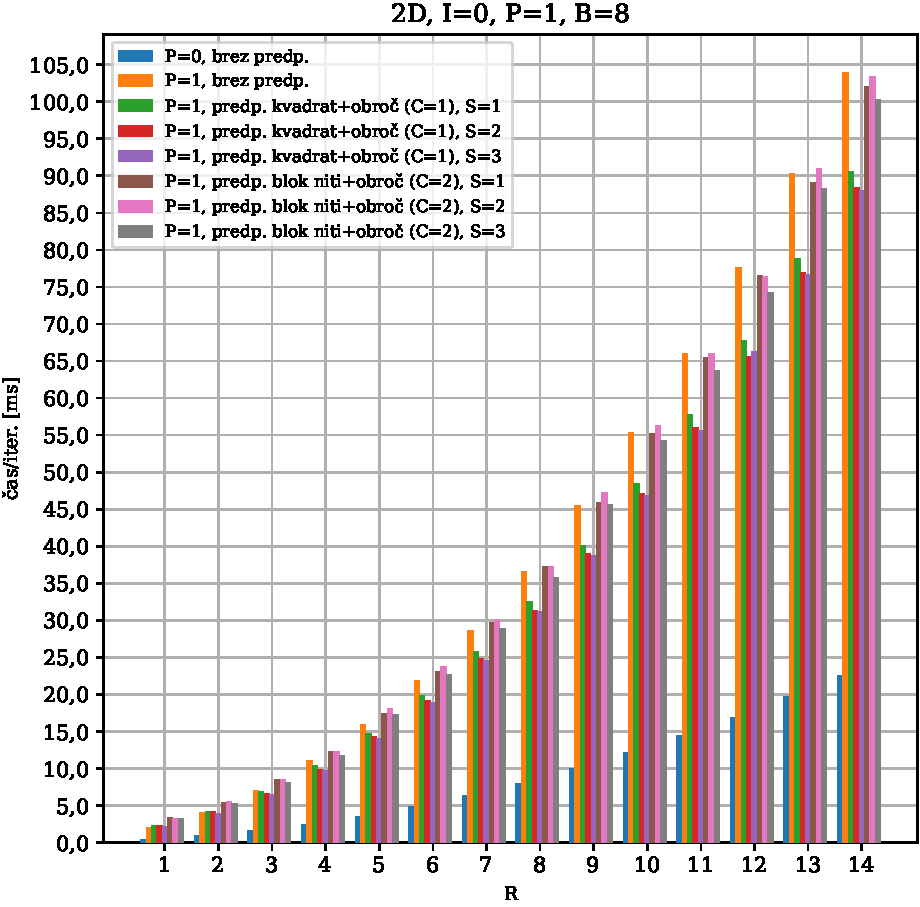
\includegraphics[width=0.7\linewidth]{images/2D_I0_P1_B8.pdf}
    \caption{Diagram časov izvajanj pri različnih soseščinah in strategijah polnjenja predpomnilnika. Velikost bloka: \(8^1\), domena niti: stolpec, sinhronizacija mreže: CPE.}
    \label{fig:2D_I0_P1_B8}
\end{figure}

\begin{figure}[H]
    \centering
    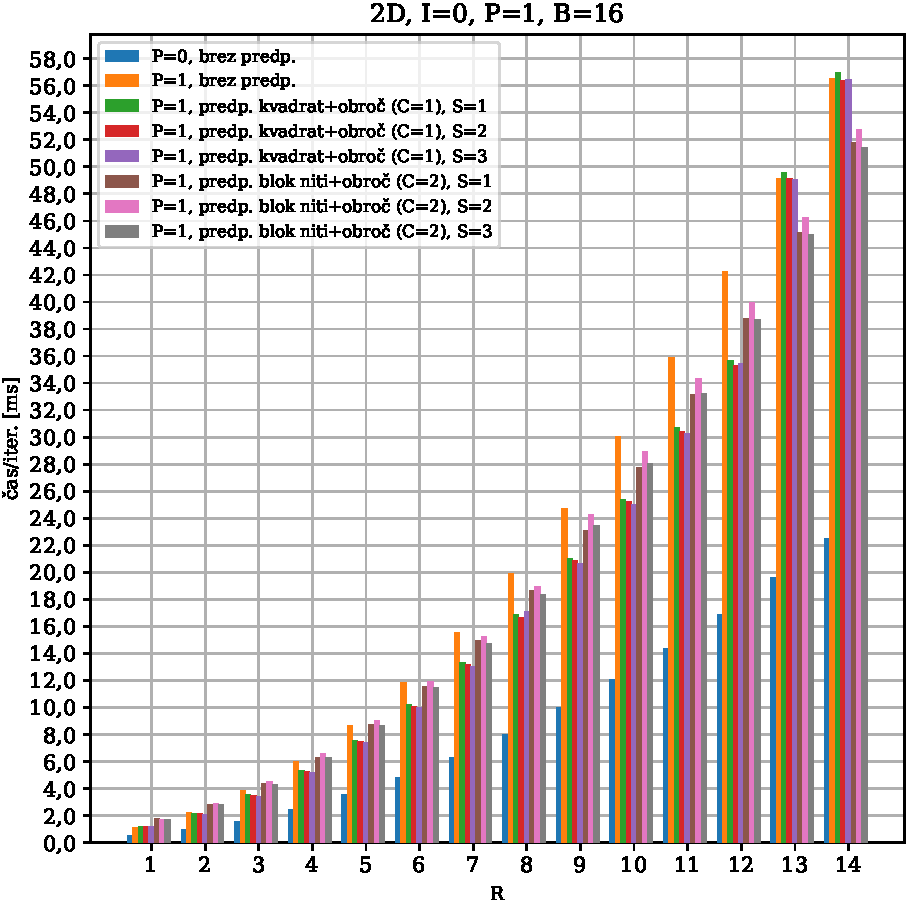
\includegraphics[width=0.7\linewidth]{images/2D_I0_P1_B16.pdf}
    \caption{Diagram časov izvajanj pri različnih soseščinah in strategijah polnjenja predpomnilnika. Velikost bloka: \(16^1\), domena niti: stolpec, sinhronizacija mreže: CPE.}
    \label{fig:2D_I0_P1_B16}
\end{figure}

% tabele
\begin{table}[H]
    \centering
    \caption{Tabela pohitritev za 2D mrežo, sinhronizacijo mreže na CPE, soseščino širine 7 in velikosti stranice bloka niti 8, za vse strategije polnjenja predpomnilnika.}
    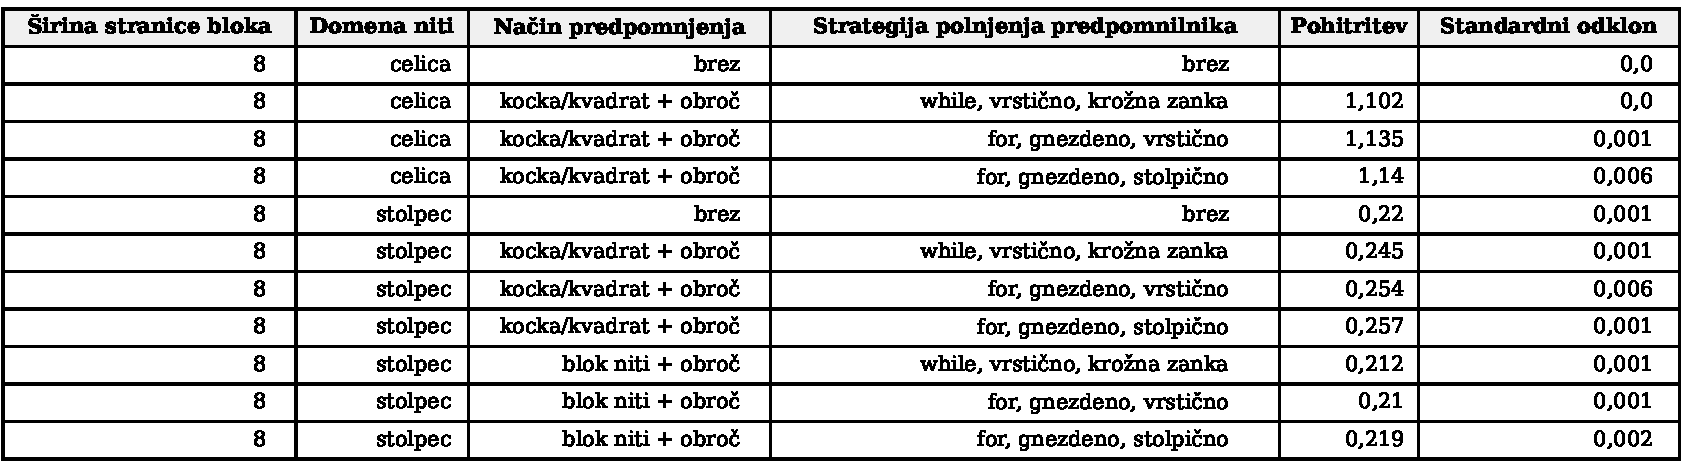
\includegraphics[width=0.9\linewidth]{tables/2D_I0_B8.pdf}
    \label{tab:2D_I0_B8}
\end{table}

\begin{table}[H]
    \centering
    \caption{Tabela pohitritev za 2D mrežo, sinhronizacijo mreže na CPE, soseščino širine 7 in velikosti stranice bloka niti 16, za vse strategije polnjenja predpomnilnika.}
    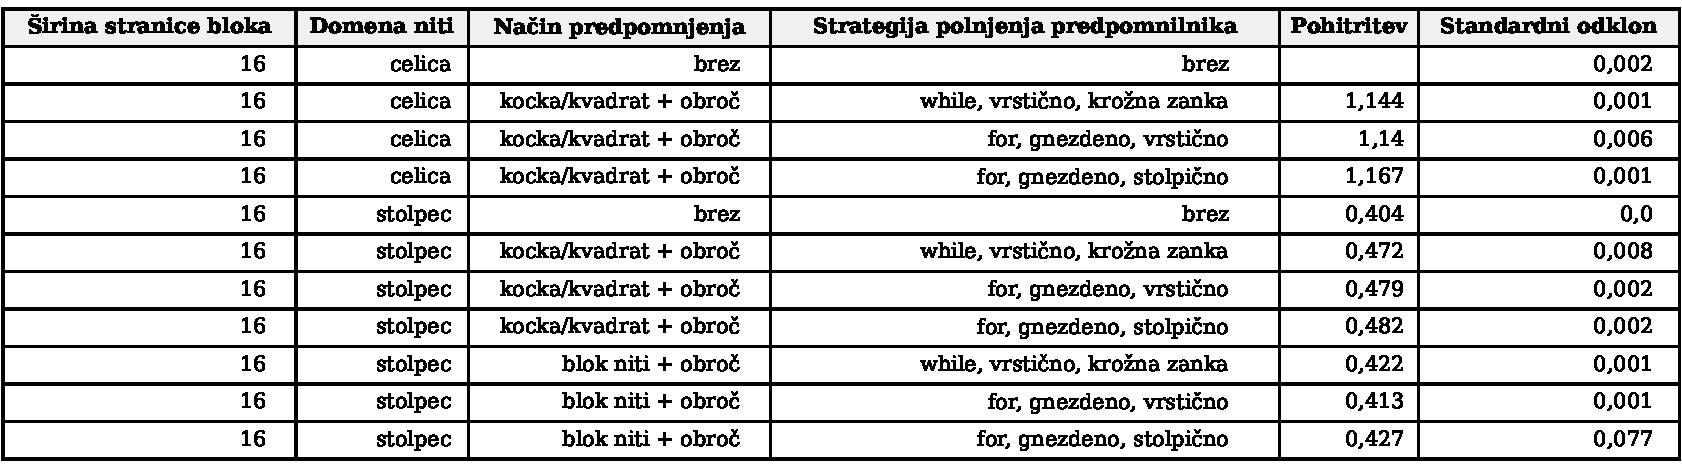
\includegraphics[width=0.9\linewidth]{tables/2D_I0_B16.pdf}
    \label{tab:2D_I0_B16}
\end{table}

\subsection{Sinhronizacija mreže preko GPE}

% 2D I1 P0
Pri sinhronizaciji mreže preko GPE (\(I=1\)) smo zaradi predhodno opisanih omejitev uporabili manjšo mrežo.
V 2D je bila ta velikosti \(W=128\) (\(128^2\) celic) - precej manjša kakor pri sinhronizaciji preko CPE.
S tem se je načeloma zmanjšal tudi čas izvajanja na iteracijo.
Največji izmerjeni standardni odklon meritev je za bloke \(B=8\) bil 0,012 ms, za \(B=16\) pa 0,034 ms.

Na diagramih \ref{fig:2D_I1_P0_B8} in \ref{fig:2D_I1_P0_B16} je mogoče opaziti podoben trend kot predhodno prikazano na \ref{fig:2D_I0_P0_B8} in \ref{fig:2D_I0_P0_B16} pri I=0: velikost bloka nima bistvenega vpliva v primerih, kjer je domena niti celica.
Čas izvajanja na iteracijo simulacije je pri primeru brez predpomnjenja pri obeh velikostih blokov približno 1,4 ms pri največji soseščini.
Prav tako je v obeh primerih precej podobno predpomnjenje kvadrata in njegovega obroča.
Strategija 1 ima za velikost bloka \(8^2\) čas izvajanja približno 0,65 ms oziroma 0,6 ms za blok \(16^2\).
Druga strategija je v obeh primerih minimalno hitrejša.
Kot je razvidno iz tabel \ref{tab:2D_I1_B8} in \ref{tab:2D_I1_B16} to prinese okoli 2-kratno pohitritev pri manjši velikosti bloka.
Pri večjem bloku je pohitritev v obeh primerih minimalno večja.
Opazno manjša pohitritev se pojavi pri tretji strategiji polnjenja predpomnilnika. Čas izvajanja na iteracijo se giblje med 1,15 in 1,2 ms pri širini soseščine 14.
Glede na logiko naslavljanja predpomnilnika je ta rezultat bolj skladen s pričakovanji kot rezultat iz konfiguracij s sinhronozacijo mreže preko CPE.
Pohitritev je tako okoli 1,14-kratna za manjši in 1,17-kratna za večji blok.

\begin{figure}[H]
    \centering
    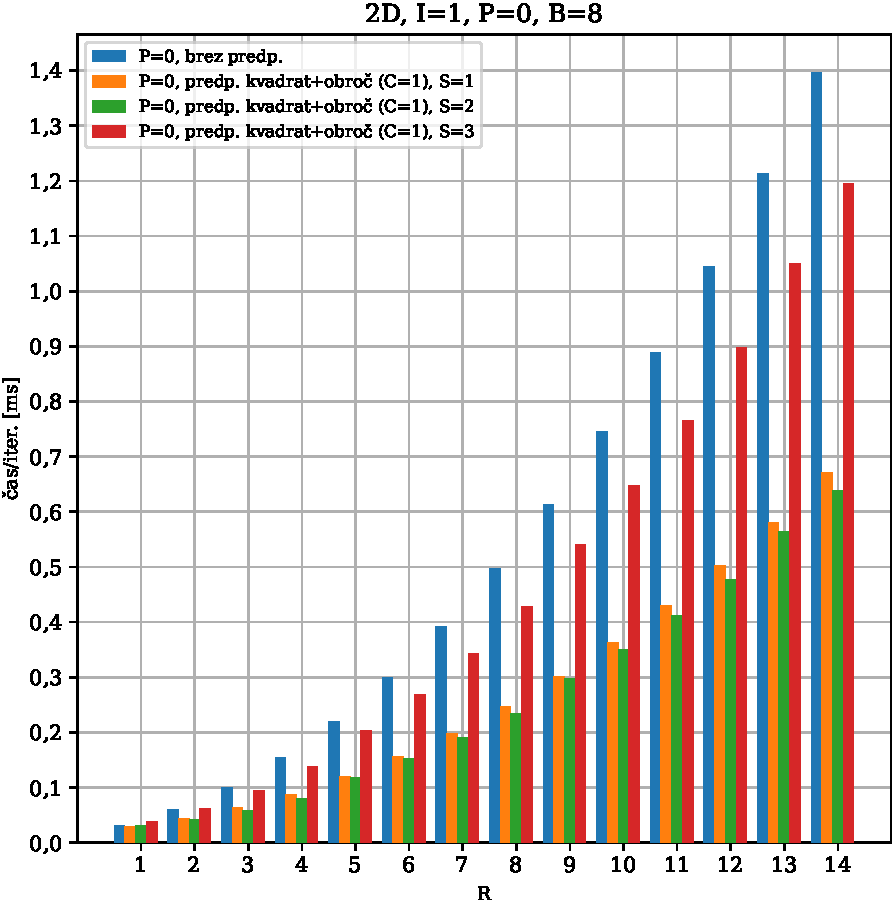
\includegraphics[width=0.7\linewidth]{images/2D_I1_P0_B8.pdf}
    \caption{Diagram časov izvajanj pri različnih soseščinah in strategijah polnjenja predpomnilnika. Velikost bloka: \(8^2\), domena niti: celica, sinhronizacija mreže: GPE.}
    \label{fig:2D_I1_P0_B8}
\end{figure}

\begin{figure}[H]
    \centering
    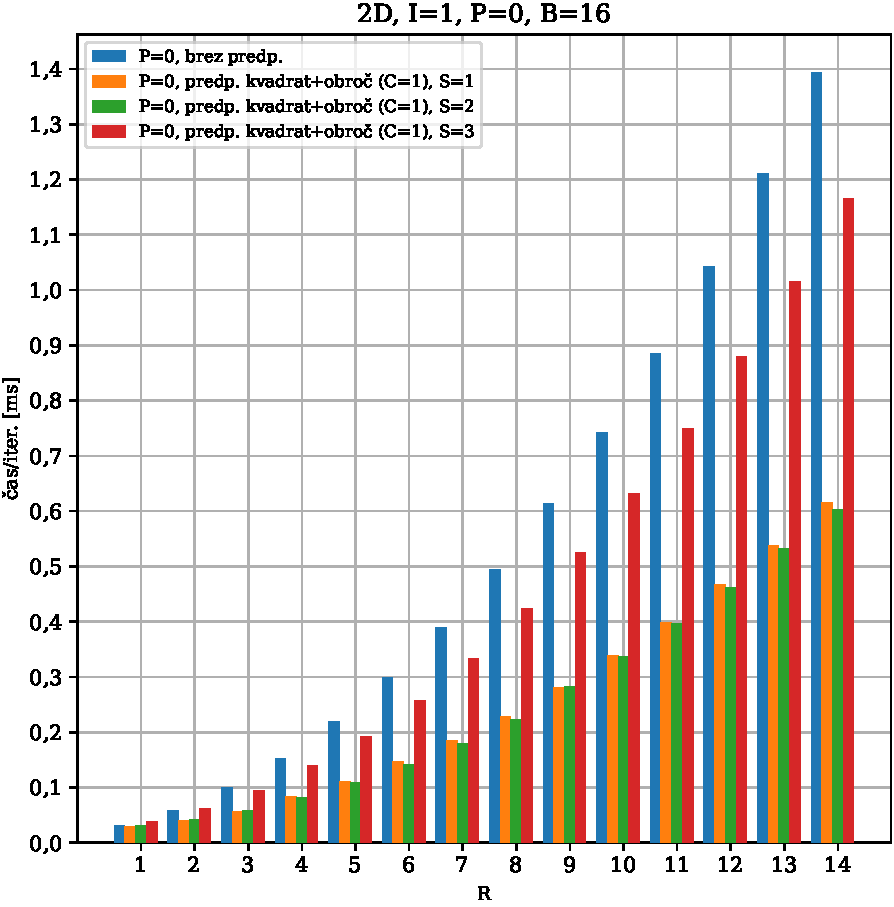
\includegraphics[width=0.7\linewidth]{images/2D_I1_P0_B16.pdf}
    \caption{Diagram časov izvajanj pri različnih soseščinah in strategijah polnjenja predpomnilnika. Velikost bloka: \(16^2\), domena niti: celica, sinhronizacija mreže: GPE.}
    \label{fig:2D_I1_P0_B16}
\end{figure}

% 2D I1 P1
Tako kot v predhodnem primeru \ref{fig:2D_I0_P1_B8}, v katerem je bila domena niti stolpec, je tudi iz diagrama \ref{fig:2D_I1_P1_B8} razvidna upočasnitev.
Ta je tokrat pri bloku \(8^1\) še nekoliko večja, skoraj 10-kratna.
Čas izvajanja na iteracijo za primer P=1 brez predpomnjenja je približno 11 ms.
Približno pol krajši so bili časi, kjer predpomnimo.
Načeloma so strategije polnjenja predpomnilnika kvadrata in obroča ponovno nekoliko hitrejše od tistih, kjer predpomnimo blok niti in obroč.
Razmerja med njimi so primerljiva s predhodno opisanimi rezultati.

Še večja upočasnitev je pri večjih blokih \(16^1\), kot je vidno iz diagrama \ref{fig:2D_I1_P1_B16}.
Dodatna upočasnitev, namesto pohitritve zaradi večjega bloka je tu bila nepričakovana in zanjo nismo našli pravega razloga.
Tudi tu je potrebno nadaljnje raziskovanje.

\begin{figure}[H]
    \centering
    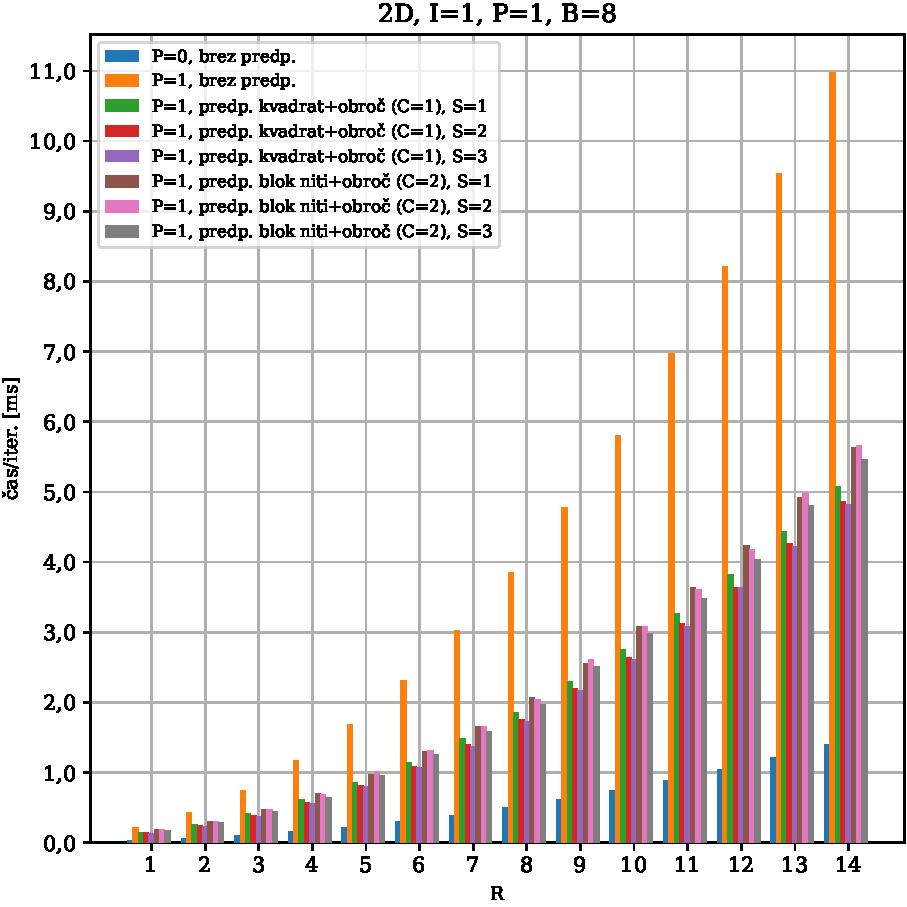
\includegraphics[width=0.7\linewidth]{images/2D_I1_P1_B8.pdf}
    \caption{Diagram časov izvajanj pri različnih soseščinah in strategijah polnjenja predpomnilnika. Velikost bloka: \(8^1\), domena niti: stolpec, sinhronizacija mreže: GPE.}
    \label{fig:2D_I1_P1_B8}
\end{figure}

\begin{figure}[H]
    \centering
    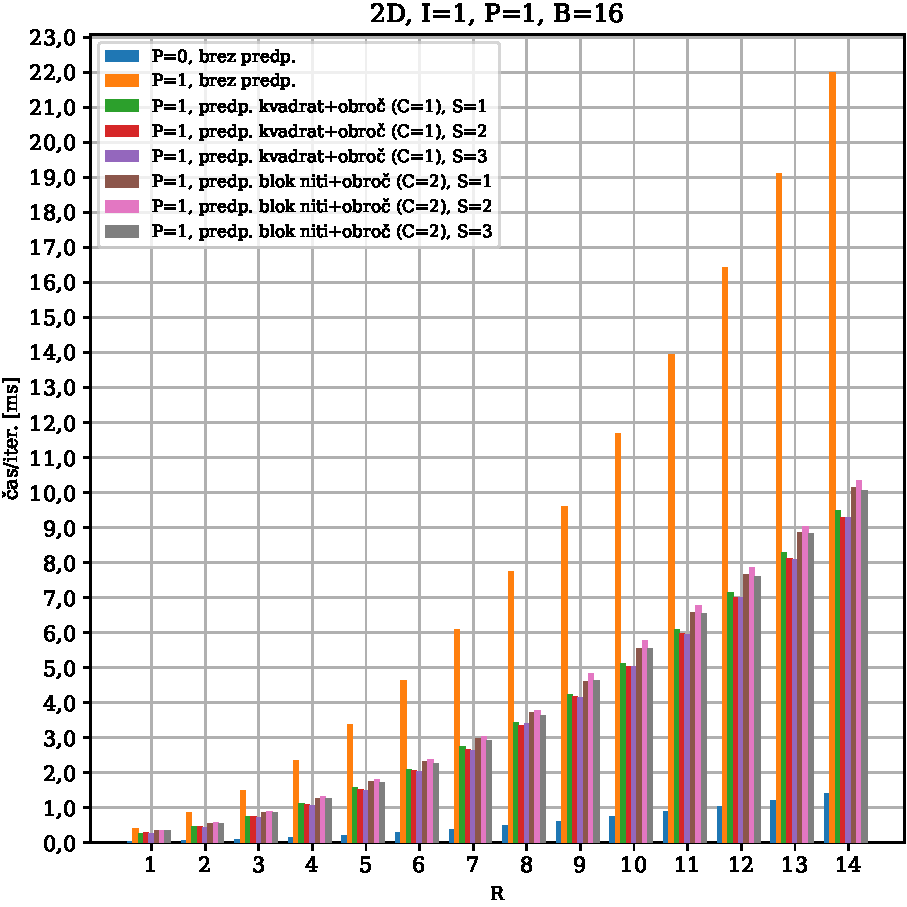
\includegraphics[width=0.7\linewidth]{images/2D_I1_P1_B16.pdf}
    \caption{Diagram časov izvajanj pri različnih soseščinah in strategijah polnjenja predpomnilnika. Velikost bloka: \(16^1\), domena niti: stolpec, sinhronizacija mreže: GPE.}
    \label{fig:2D_I1_P1_B16}
\end{figure}

% tabele
\begin{table}[H]
    \centering
    \caption{Tabela pohitritev za 2D mrežo, sinhronizacijo mreže na GPE, soseščino širine 7 in velikosti stranice bloka niti 8, za vse strategije polnjenja predpomnilnika.}
    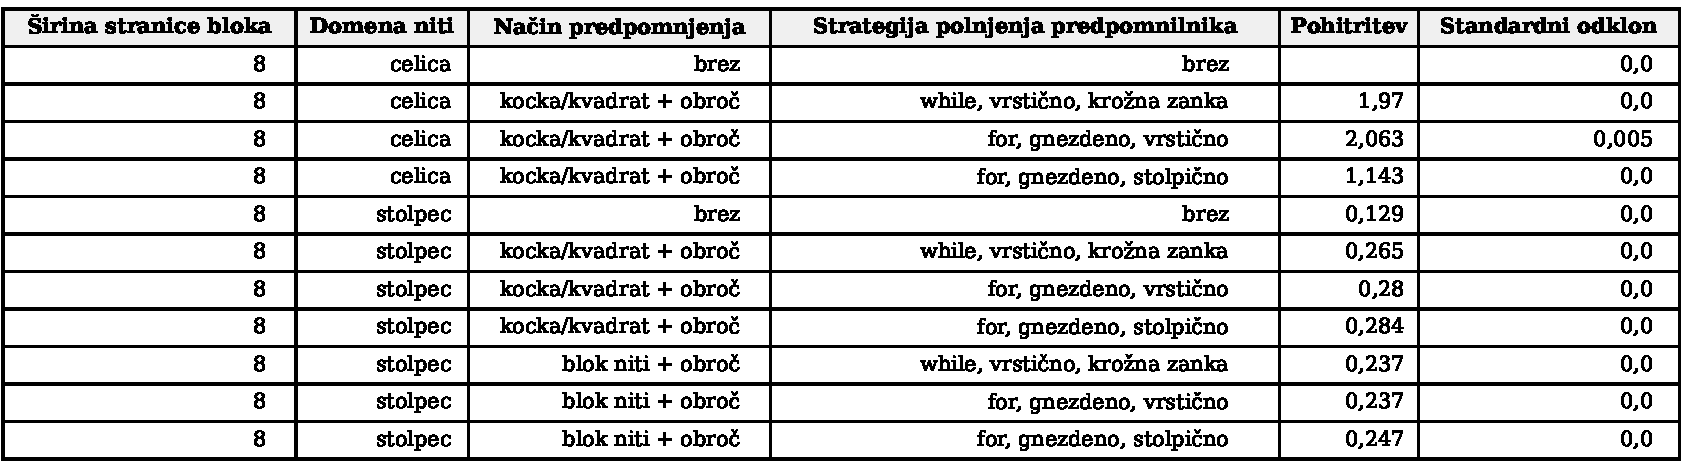
\includegraphics[width=0.9\linewidth]{tables/2D_I1_B8.pdf}
    \label{tab:2D_I1_B8}
\end{table}

\begin{table}[H]
    \centering
    \caption{Tabela pohitritev za 2D mrežo, sinhronizacijo mreže na GPE, soseščino širine 7 in velikosti stranice bloka niti 16, za vse strategije polnjenja predpomnilnika.}
    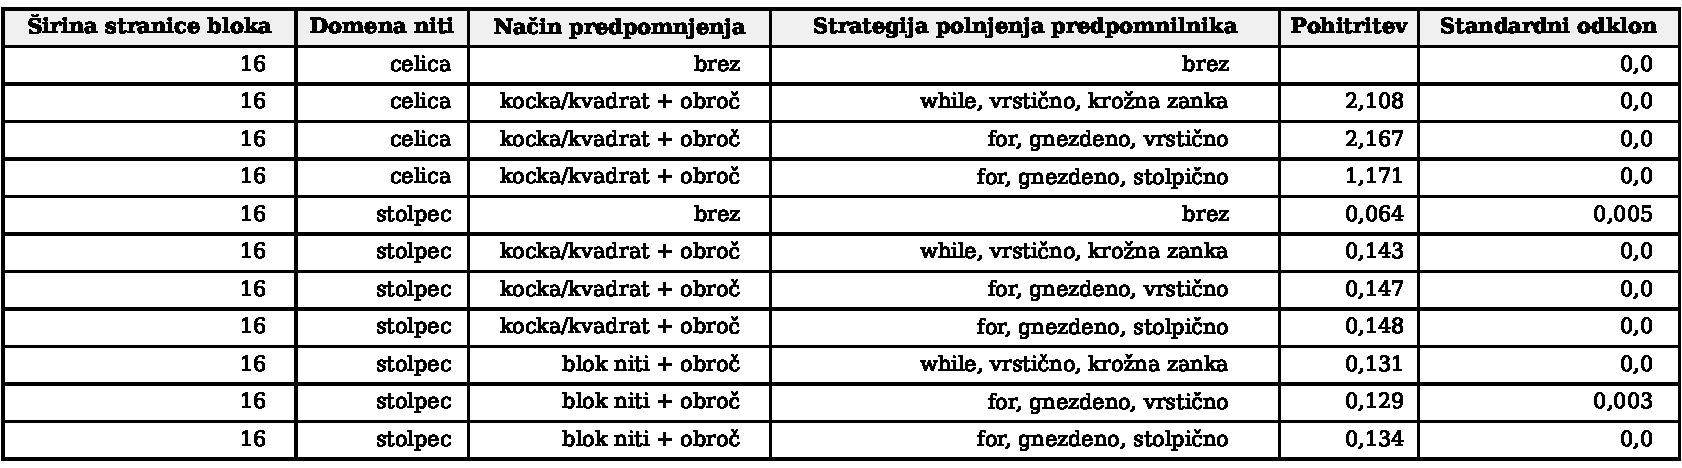
\includegraphics[width=0.9\linewidth]{tables/2D_I1_B16.pdf}
    \label{tab:2D_I1_B16}
\end{table}

\section{3D}

V trodimenzionalni mreži smo izbrali manjše velikosti stranic blokov niti: \(B=4\) in \(B=8\).
3D bloki so imeli \(4^3\) oziroma \(8^3\) celic pri domeni niti ene celice (\(P=0\)) in \(4^2\) ter \(8^2\) celic v primeru, ko je domena niti stolpec (\(P=1\)).

\subsection{Sinhronizacija mreže preko CPE}

% 3D I0 P0 B4
Pri sinhronizaciji mreže preko CPE (\(I=0\)) v 3D okolju smo za simulacije izbrali velikost mreže \(W=128\) (\(128^3\) celic).
Največji standardni odklon meritev je pri \(B=4\) bil 2,882 ms, pri \(B=8\) pa 3,470 ms.

Tu je bilo prvič mogoče opaziti omejitev soseščine zaradi velikosti dodeljenega skupnega pomnilnika.
Kot je razvidno iz diagrama \ref{fig:3D_I0_P0_B4}, je pri domeni niti ene celice največja dovoljena soseščina pri bloku \(4^3\) bila 9, ko želimo predpomniti kocko in njen obroč.
Kombinacija predpomnenja in tako široke soseščine daje velikost skupnega pomnilnika \((9 \times 2 + 4)^3\), kar pri velikosti posameznega podatka v celici 4 B, prinese nekaj več kot 41,4 kB porabljenega skupnega pomnilnika.
Če bi bila soseščina še za eno celico večja, bi bilo porabljenega že 54 kB, pri omejitvi 48 kB na blok niti.

Poleg omejitve velikosti skupnega pomnilnika je moč opaziti tudi eksponentno slabšanje časov izvajanj na iteracijo primerov, kjer predpomnimo, glede na osnovno konfiguracijo brez predpomnjenja.
Pri največji še mogoči soseščini za predpomnjenje, R=9, je tako opazna nekajkratna upočasnitev.

Razlog v eksponentni upočasnitvi vidimo v količini dela, ki ga mora vsaka nit v bloku opraviti pri polnjenju skupnega pomnilnika. Večja kot je soseščina, večji delež volumna v predpomnilniku predstavljajo celice iz obroča.
Pri R=4, bo predpomnilnik moral zadostovati \(12^3\) celicam, pri R=9 pa \(22^3\) celicam.
Če takšen volumen primerjamo z blokom niti velikosti \(4^3\), opazimo, da se delo vsake niti s povečevanjem soseščine eksponentno povečuje.

Sicer je čas izvajanja na iteracijo pri konfiguraciji brez predpomnjenja pri največji širini soseščine približno 390 ms, pri največji dovoljeni soseščini za predpomnjenje pa so časi izvajanj za konfiguracije s predpomnjenjem okoli 350-370 ms.
Opaziti je mogoče približno enake čase izvajanj na iteracijo za strategije 1 in 3, medtem ko je strategija 2 nekoliko hitrejša.

\begin{figure}[H]
    \centering
    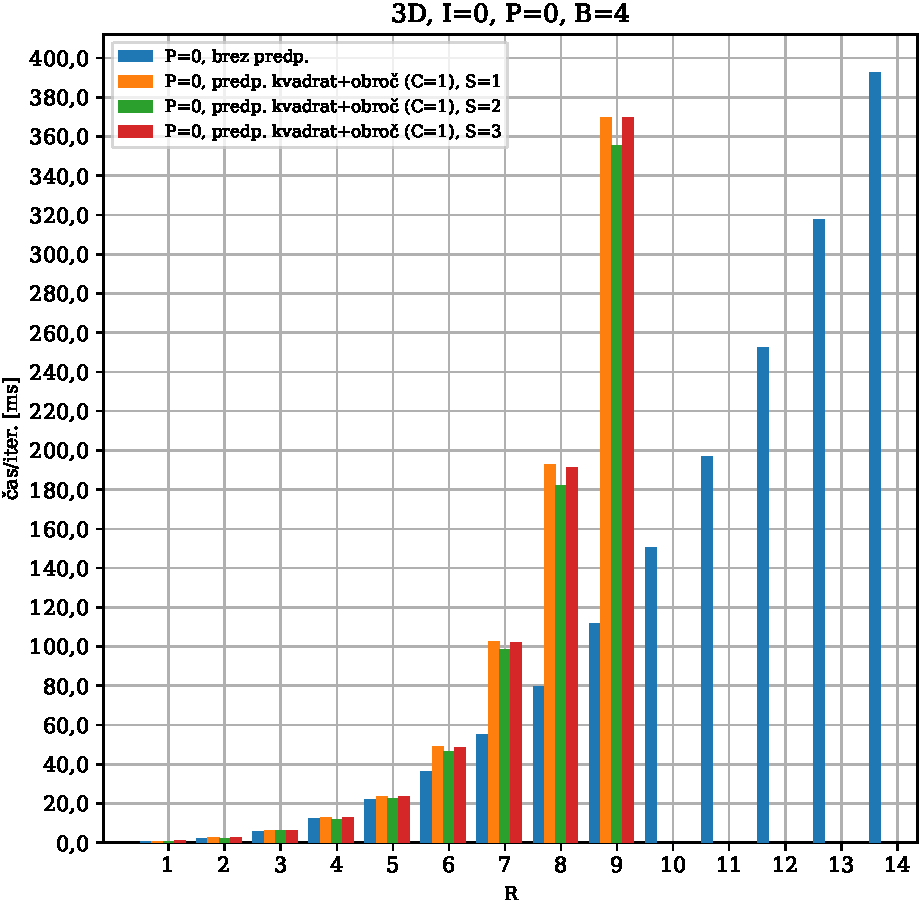
\includegraphics[width=0.7\linewidth]{images/3D_I0_P0_B4.pdf}
    \caption{Diagram časov izvajanj pri različnih soseščinah in strategijah polnjenja predpomnilnika. Velikost bloka: \(4^3\), domena niti: celica, sinhronizacija mreže: CPE.}
    \label{fig:3D_I0_P0_B4}
\end{figure}

% 3D I0 P1 B4
Omejitve velikosti predpomnilnika se spet spremenijo, ko za domeno niti uporabimo stolpec.
Iz diagrama \ref{fig:3D_I0_P1_B4} je razvidna različna zgornja meja velikosti soseščine pri različnih načinih predpomnjenja.
Predpomnjenje kocke in obroča dovoljuje največjo širino soseščine 9, medtem ko je pri predpomnjenju le bloka in obroča minimalno večja, R=10.

Čas izvajanja na iteracijo pri različici brez predpomnjenja je pri največji soseščini približno 910 ms, kar pomeni 0,4-kratno pohitritev, torej skoraj dvokratno upočasnitev, kot je razvidno iz tabele \ref{tab:3D_I0_B4}.

Strategije polnjenja predpomnilnika kocke in obroča pri njihovi največji soseščini R=9 dosegajo čase izvajanja na iteracijo od 1400 do 1550 ms.
Najhitrejša je druga strategija, medtem ko sta prva in tretja načeloma na enaki ravni.
Časi izvajanj prinašajo okoli 14-kratno upočasnitev glede na osnovno konfiguracijo.
Za približno 100 ms na iteracijo so pri R=9 počasnejše konfiguracije s predpomnjenjem bloka niti in obroča.
Te pri svoji največji soseščini dosegajo čase izvajanj od 2500 do 2600 ms.
Pri največji soseščini je najpočasnejša strategija 1, medtem ko sta druga in tretja približno enako hitri. Razlika je pri manjših soseščinah, kjer so manjše razlike med najhitrejšo in najpočasnejšo strategijo.

Pri tolmačenju teh upočasnitev je potrebno izpostaviti velikost bloka, ki je pri P=1 v tem primeru \(4^2\).
To znaša le polovico enega snopa, kar spet privede do polovice neuporabljenih niti znotraj snopa ter posledično do upočasnitve.

\begin{figure}[H]
    \centering
    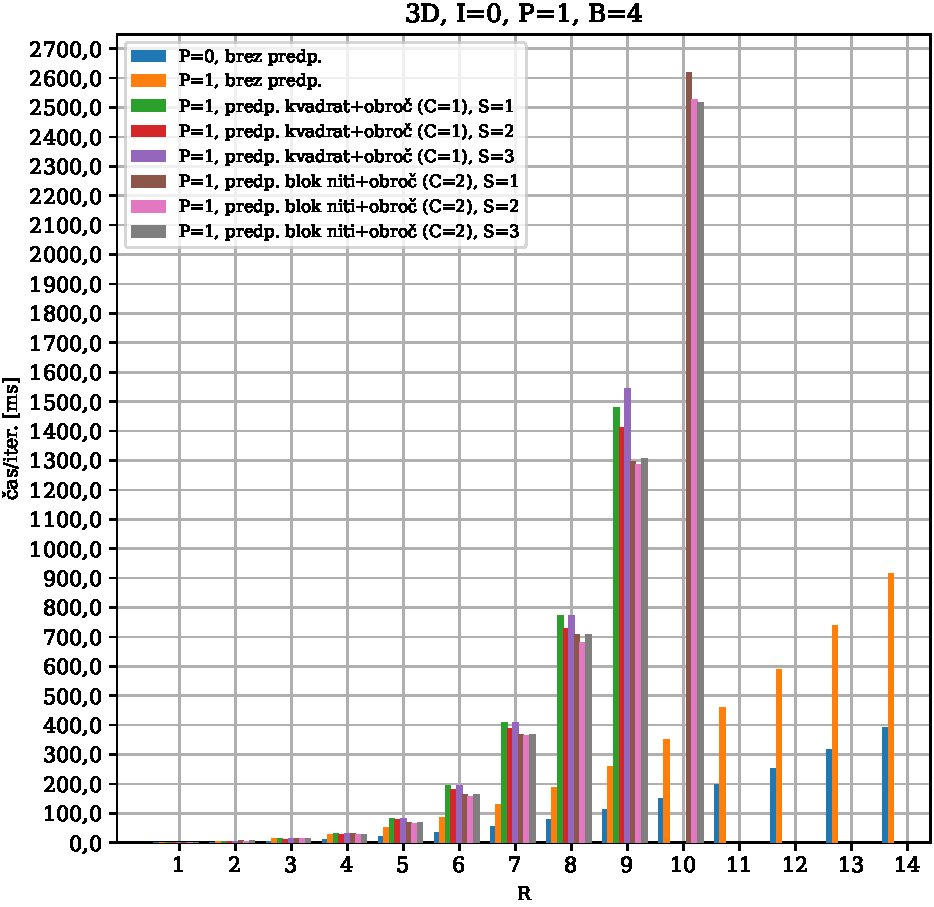
\includegraphics[width=0.7\linewidth]{images/3D_I0_P1_B4.pdf}
    \caption{Diagram časov izvajanj pri različnih soseščinah in strategijah polnjenja predpomnilnika. Velikost bloka: \(4^2\), domena niti: stolpec, sinhronizacija mreže: CPE}
    \label{fig:3D_I0_P1_B4}
\end{figure}

\begin{table}[H]
    \centering
    \caption{Tabela pohitritev za 3D mrežo, sinhronizacijo mreže na CPE, soseščino širine 7 in velikosti stranice bloka niti 4, za vse strategije polnjenja predpomnilnika.}
    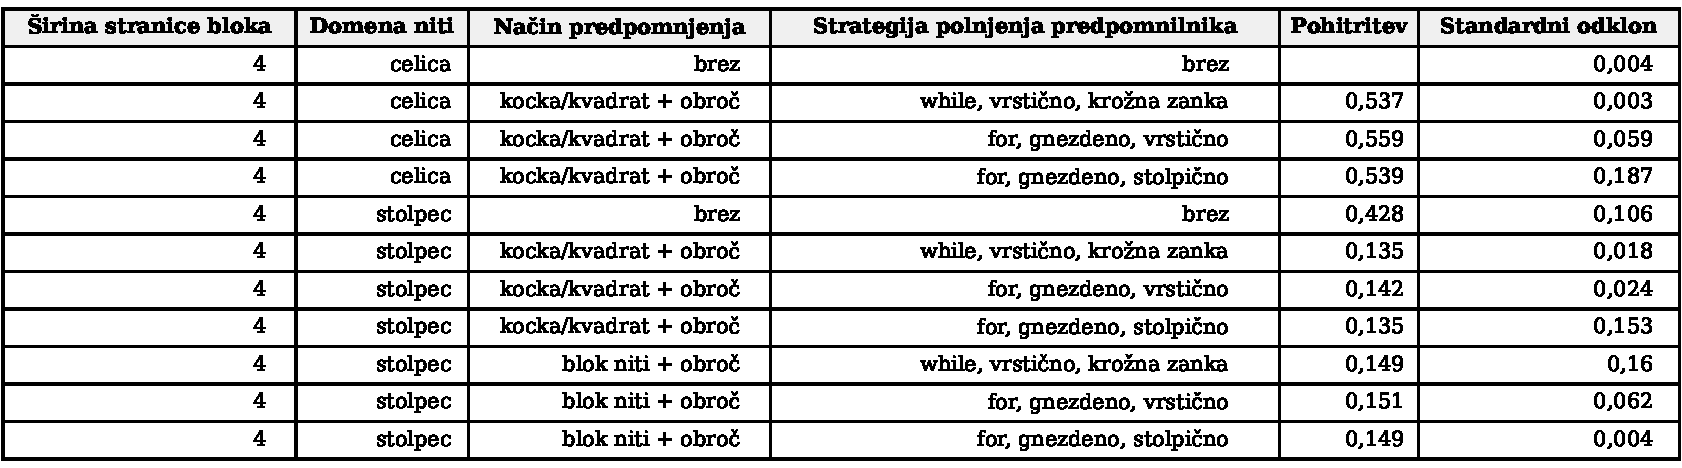
\includegraphics[width=0.9\linewidth]{tables/3D_I0_B4.pdf}
    \label{tab:3D_I0_B4}
\end{table}

% 3D I0 P0 B8
Ko povečamo blok na \(8^3\) in za domeno niti postavimo celico, se omejitev širine soseščine še zmanjša. Iz diagrama \ref{fig:3D_I0_P0_B8} je vidna omejitev pri R=7. Pri tej soseščini imamo v skupnem pomnilniku \(22^3 = 10648\) celic, oziroma nekaj več kot 41,5 kB zasedenega skupnega pomnilnika za vsak blok niti.

Opaziti je mogoče tudi rahlo počasnejše čase izvajanj pri osnovni konfiguraciji brez predpomnjenja. Pri največji soseščini je čas izvajanja na iteracijo okoli 450 ms - pri manjših blokih \(4^3\) je ta čas 390 ms.

Nasprotno je mogoče opaziti pri časih izvajanj na iteracijo, kjer predpomnimo.
Predpomnilne strategije so si sicer enakovredne z minimalnimi razlikami, a v primerjavi s konfiguracijimi z manjšimi bloki so hitrejše od osnovne konfiguracije.
Iz tabele \ref{tab:3D_I0_B8} je videti pri njihovi največji soseščini okoli 1,15-kratne pohitritve.

Pomembno je izpostaviti, da pri večjih blokih \(8^3\) obroči predstavljajo manjši delež celotnega volumna v skupnem pomnilniku kot pri manjših blokih.
To pomeni nekoliko manj dela za vsako nit v bloku, kar se lahko odraža v časih izvajanj.

\begin{figure}[H]
    \centering
    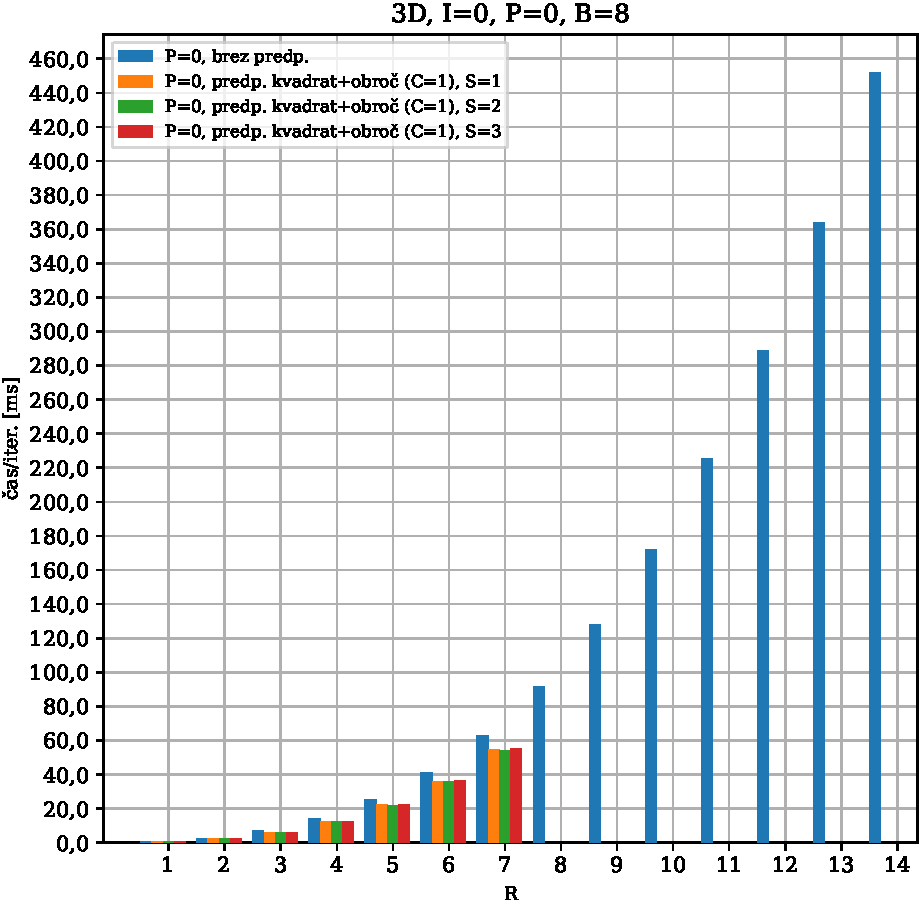
\includegraphics[width=0.7\linewidth]{images/3D_I0_P0_B8.pdf}
    \caption{Diagram časov izvajanj pri različnih soseščinah in strategijah polnjenja predpomnilnika. Velikost bloka: \(8^3\), domena niti: celica, sinhronizacija mreže: CPE.}
    \label{fig:3D_I0_P0_B8}
\end{figure}

% 3D I0 P1 B8
Ko pri B=8 za domeno niti postavimo stolpec, se blok iz treh dimenzij zmanjša na \(8^2\) in s tem tudi prvič dobimo za P=1 bloke niti, ki so veliki za vsaj en snop. V tem primeru bodo bloki veliki dva snopa.
Na podlagi tega pričakujemo, da bodo konfiguracije z domeno niti enako stolpcu prvič hitrejše kakor osnovne konfiguracije brez predpomnjenja in z domeno niti enako celici.

Iz diagrama \ref{fig:3D_I0_P1_B8} je ta predpostavka razvidna, a le pri konfiguraciji brez predpomnjenja.
Pri največji soseščini ima tako različica brez predpomnjenja in z domeno niti enako stolpcu nekoliko hitrejši čas izvajanja na iteracijo kot osnovna konfiguracija.
Hitrejša je za okoli 30 ms na iteracijo, pohitritev je okoli 1,07-kratna.

Konfiguracije s predpomnjenjem imajo enake omejitve soseščine, kot že opaženo pri manjših blokih, so pa počasnejše kot konfiguracije brez predpomnjenja. Pri R=7 so časi izvajanj konfiguracij s predpomnjenjem kocke in obroča 185-190 ms na iteracijo, kar pomeni pohitritve z vrednostjo okoli 0,033.

Strategije \hfill polnjenja \hfill predpomnilnika \hfill bloka \hfill niti \hfill in \hfill obroča \hfill so \hfill pri \hfill isti \\
soseščini vidno hitrejše, a še vedno s pohitritvami, manjšimi od 1.
Kot je razvidno iz tabele \ref{tab:3D_I0_B8}, so pohitritve približno 0,43-kratne.

Pri vseh strategijah polnjenja predpomnilnika je druga strategija minimalno hitrejša od drugih dveh, ki pa sta na približno enaki ravni.

Da so rezultati konfiguracij s predpomnjenjem počasnejši od tistih brez, je nepričakovano, zato bi tudi tu bilo potrebno nadaljnje raziskovanje.

\begin{figure}[H]
    \centering
    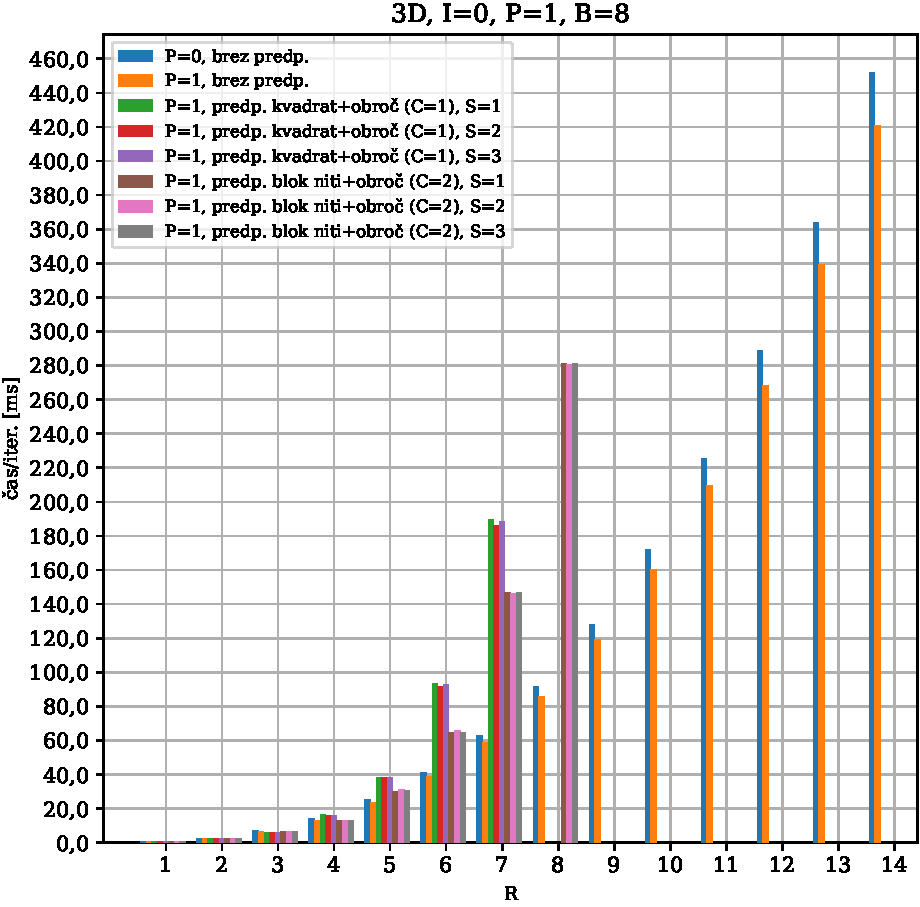
\includegraphics[width=0.7\linewidth]{images/3D_I0_P1_B8.pdf}
    \caption{Diagram časov izvajanj pri različnih soseščinah in strategijah polnjenja predpomnilnika. Velikost bloka: \(8^2\), domena niti: stolpec, sinhronizacija mreže: CPE.}
    \label{fig:3D_I0_P1_B8}
\end{figure}

\begin{table}[H]
    \centering
    \caption{Tabela pohitritev za 3D mrežo, sinhronizacijo mreže na CPE, soseščino širine 7 in velikosti stranice bloka niti 8, za vse strategije polnjenja predpomnilnika.}
    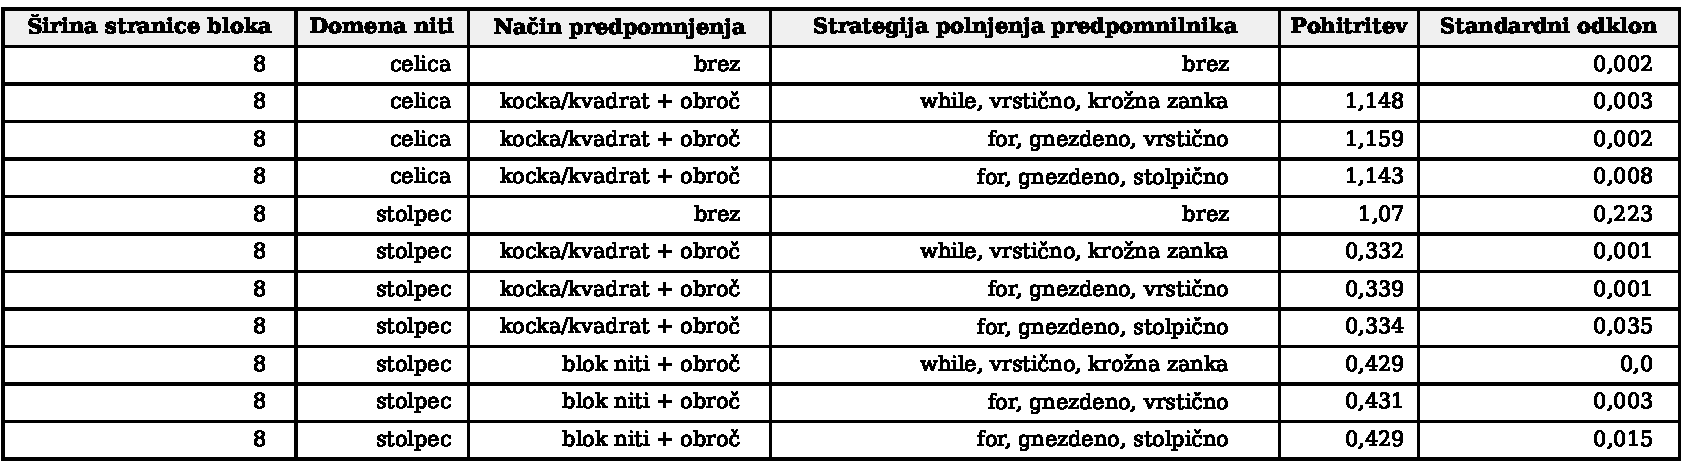
\includegraphics[width=0.9\linewidth]{tables/3D_I0_B8.pdf}
    \label{tab:3D_I0_B8}
\end{table}

\subsection{Sinhronizacija mreže preko GPE}

Za velikost 3D mreže, sinhronizirane preko GPE (\(I=1\)), smo za njeno velikost izbrali \(W=32\), kar je prineslo \(32^3\) celic.
Pri \(B=4\) je največji izmerjeni standardni odklon bil 0,475 ms, pri \(B=8\) pa 0,263 ms.

% 3d i1 p0 B4
Pri domeni niti ene celice z bloki velikosti \(4^3\), je vidna pohitritev namesto upočasnitve, kot prikazano na diagramu \ref{fig:3D_I1_P0_B4}.
Konfiguracija brez predpomnjenja pri največji soseščini doseže čas izvajanja na iteracijo skoraj 43 ms. To je neprimerljivo manj kakor pri ekvivalentni konfiguraciji pri sinhronizaciji mreže preko CPE, kjer je tudi mreža bila neprimerna večja.

Omejitev za blok \(4^3\) je še vedno smiselna pri R=9, časi izvajanj na iteracijo za konfiguracije s predpomnjenjem so okoli dvakrat hitrejši kakor v osnovni konfiguraciji, kar je tudi razvidno iz tabele \ref{tab:3D_I1_B4}.

Od \hfill strategij \hfill polnjenja \hfill predpomnilnika \hfill je \hfill prva \hfill strategija \hfill spet \\
najpočasnejša, druga in tretja sta rahlo hitrejši.
Med slednjima opaziti pomembnih razlik.

Ker je 3D mreža veliko manjša in s tem manjše število vseh blokov niti, smo se s tem znebili morebitnih čakanj blokov na izvajanje na računskih enotah.
Predvidevamo, da so pri večji mreži nekateri bloki morali čakati na izvajanje, ker so bile računske enote prezasedene, kar lahko ohromi zmogljivost.

\begin{figure}[H]
    \centering
    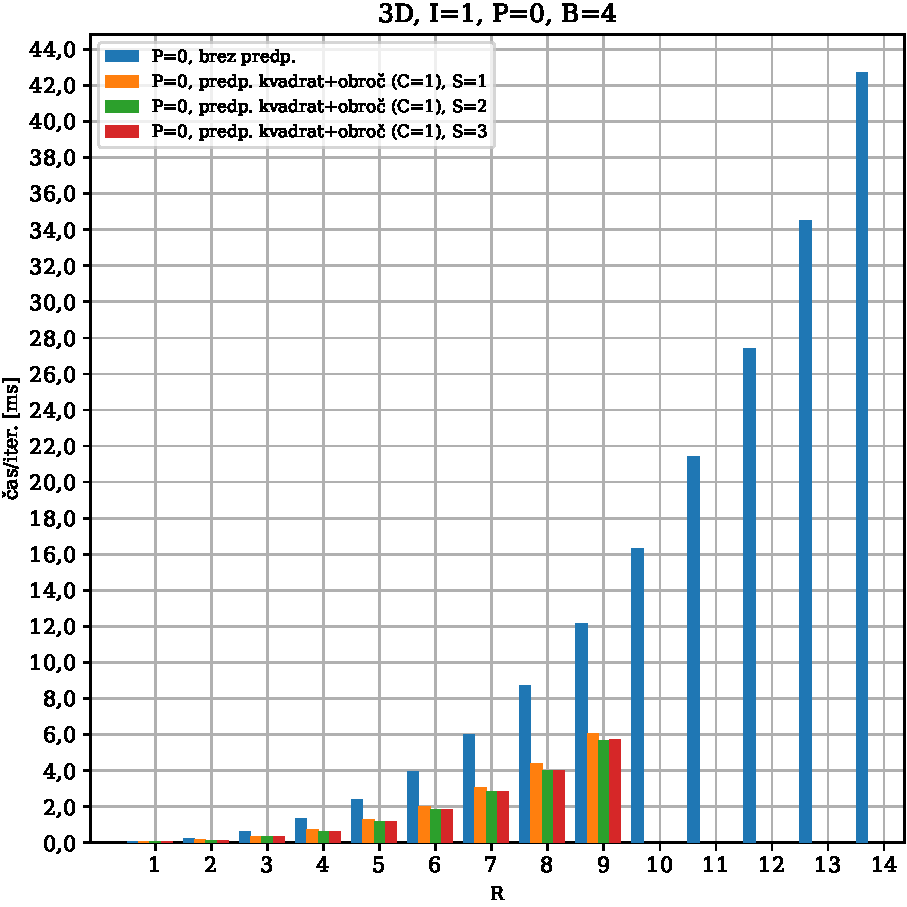
\includegraphics[width=0.7\linewidth]{images/3D_I1_P0_B4.pdf}
    \caption{Diagram časov izvajanj pri različnih soseščinah in strategijah polnjenja predpomnilnika. Velikost bloka: \(4^3\), domena niti: celica, sinhronizacija mreže: GPE.}
    \label{fig:3D_I1_P0_B4}
\end{figure}

% 3d i1 p1 B4
Ko za domeno niti določimo stolpec, pride spet do upočasnitve, kot razvidno iz diagrama \ref{fig:3D_I1_P1_B4}.
Pri največji soseščini je za konfiguracijo brez predpomnjenja vidna približno štirikratna upočasnitev.
Enako velja za manjše soseščine, razvidno tudi iz tabele \ref{tab:3D_I1_B4}.

Manjše, približno dvokratne upočasnitve so za konfiguracije s predpomnjenjem, kjer prav tako ni mogoče videti večjih razlik med njimi.
Načeloma sta oba načina predpomnjenja približno enako hitra, razlika je le v največji možni soseščini.

Med strategijami polnjenja predpomnilnika ima rahlo prednost druga strategija, medtem ko sta prva in tretja enakih hitrosti.

Ker gre za bloke \(4^2\), torej velikosti polovice snopa, so takšne upočasnitve pričakovane.

Če primerjamo te rezultate s tistimi za konfiguracije, kjer je sinhronizacija mreže izvedena preko CPE, je za razliko od slednje, pri sinhronizaciji na GPE mogoče videti pohitritve načinov s predpomnjenjem glede na način brez predpomnjenja in z domeno niti enako stolpcu.

\begin{figure}[H]
    \centering
    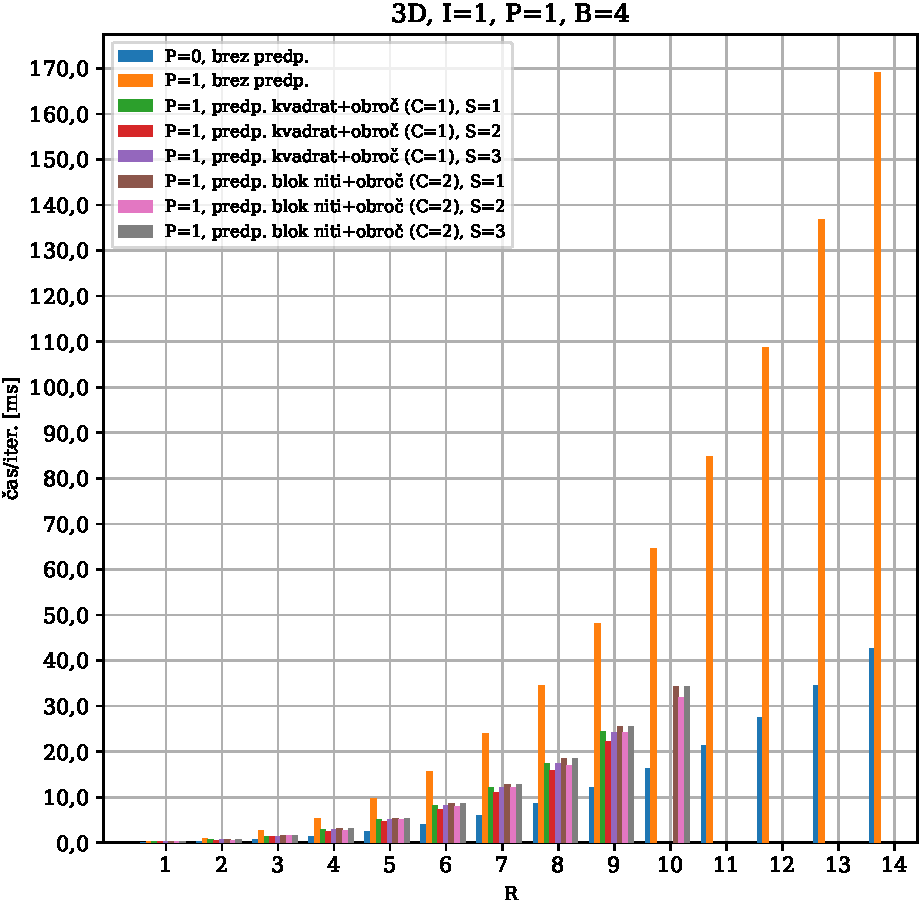
\includegraphics[width=0.7\linewidth]{images/3D_I1_P1_B4.pdf}
    \caption{Diagram časov izvajanj pri različnih soseščinah in strategijah polnjenja predpomnilnika. Velikost bloka: \(4^2\), domena niti: stolpec, sinhronizacija mreže: GPE.}
    \label{fig:3D_I1_P1_B4}
\end{figure}

\begin{table}[H]
    \centering
    \caption{Tabela pohitritev za 3D mrežo, sinhronizacijo mreže na GPE, soseščino širine 7 in velikosti stranice bloka niti 4, za vse strategije polnjenja predpomnilnika.}
    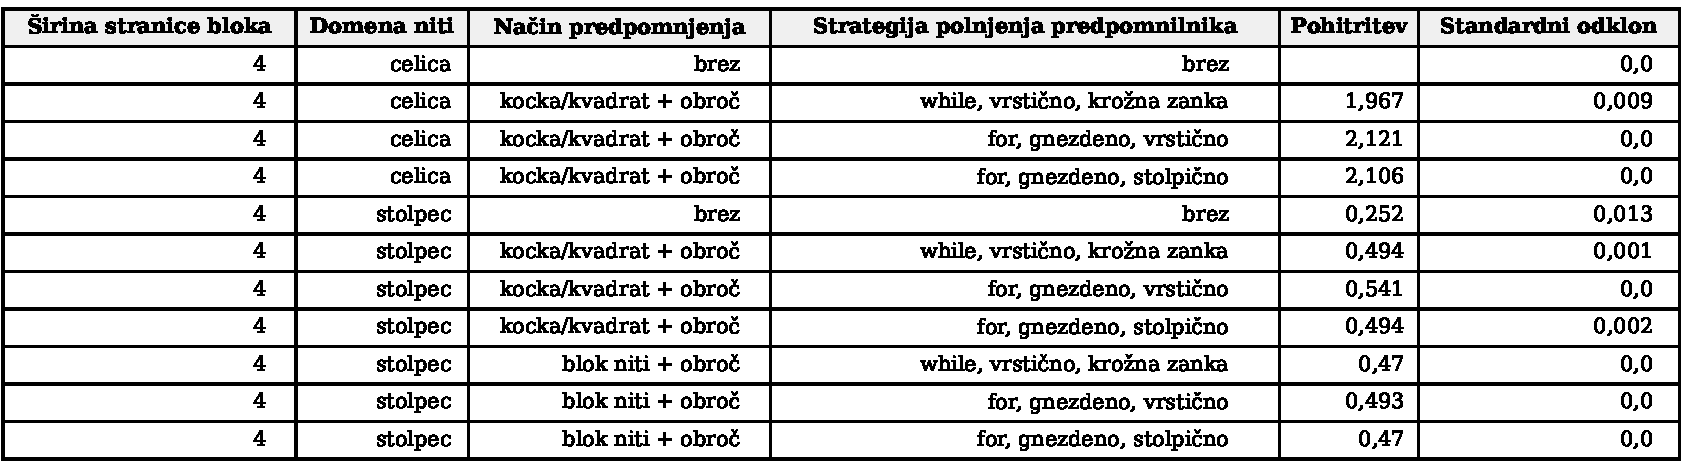
\includegraphics[width=0.9\linewidth]{tables/3D_I1_B4.pdf}
    \label{tab:3D_I1_B4}
\end{table}

% 3d i1 p0 b8
Ob povečavi bloka na \(8^3\) in domeni niti celice je iz diagrama \ref{fig:3D_I1_P0_B8} razvidno, da velikost bloka nima vpliva na čase izvajanj na iteracijo, ko gre za domeno niti celice.
Časi vseh konfiguracij so skoraj identični tistim pri manjših blokih.
Razlika se pojavi v omejitvi velikosti skupnega pomnilnika, ker je največja širina soseščine 7.

Med strategijami polnjenja predpomnilnika ni opaziti razlik.

\begin{figure}[H]
    \centering
    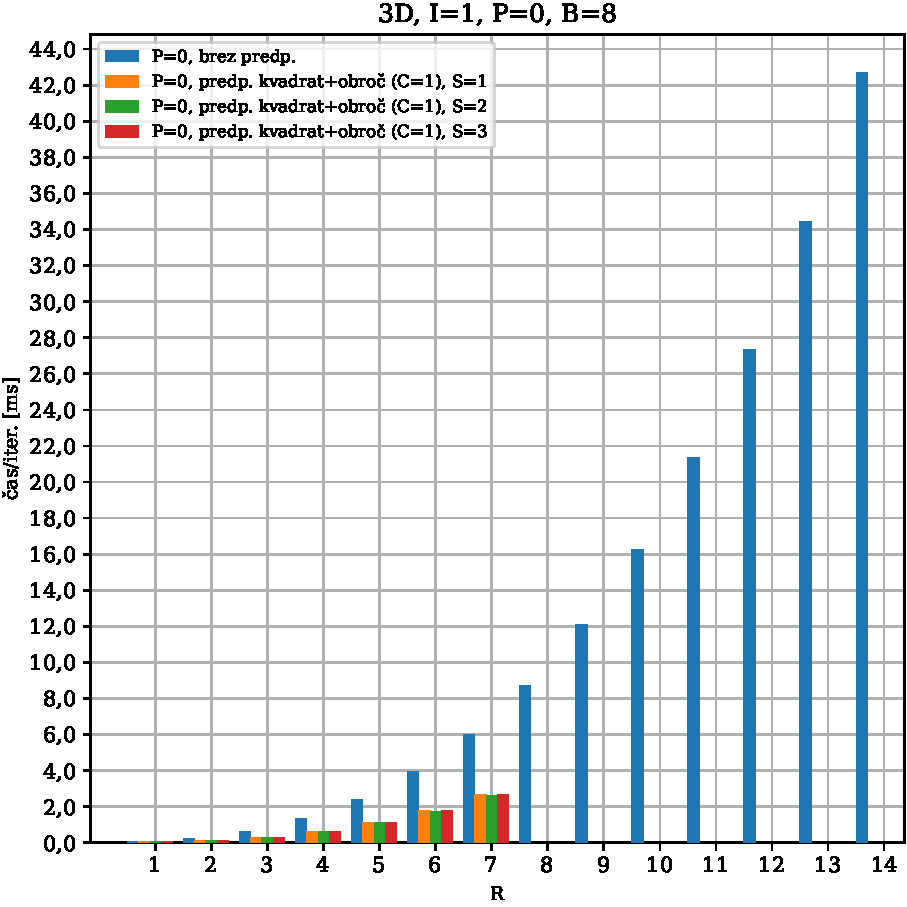
\includegraphics[width=0.7\linewidth]{images/3D_I1_P0_B8.pdf}
    \caption{Diagram časov izvajanj pri različnih soseščinah in strategijah polnjenja predpomnilnika. Velikost bloka: \(8^3\), domena niti: celica, sinhronizacija mreže: GPE.}
    \label{fig:3D_I1_P0_B8}
\end{figure}

% 3d i1 p1 b8
Ko konfiguracijam s parametrom B=8 določimo še domeno niti na stolpec, se rezultati obrnejo, kot razvidno iz diagrama \ref{fig:3D_I1_P1_B8}.
Pričakovane so bile pohitritve, ker imamo bloke velikosti dveh dveh snopov.
Namesto pohitritve je pri konfiguraciji brez predpomnjenja pri največji soseščini čas izvajanja na iteracijo okoli 335 ms, kar je okoli 8-krat počasneje kot pri osnovni konfiguraciji.

Kot je mogoče razbrati iz tabele \ref{tab:3D_I1_B8}, so upočasnitve pri konfiguracijah s predpomnjenjem manjše, približno 3,5-kratne s faktorjem pohitritve okoli 0,28.
Razlike med načini in strategijami polnjenja predpomnilnika so videti zanemarljive.

Rezultati so nepričakovani, tudi glede na predhodno izpostavljena odstopanja predstavljajo največjo anomalijo, ki bi jo bilo potrebno raziskati v nadaljnjih raziskavah.

\begin{figure}[H]
    \centering
    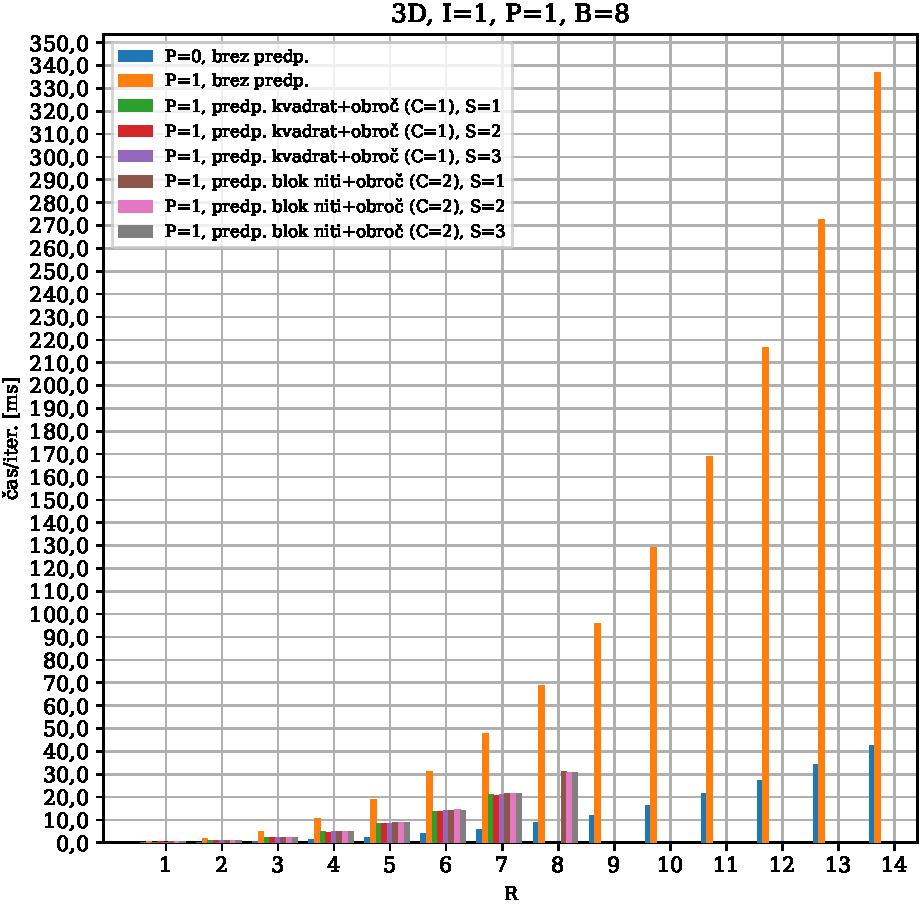
\includegraphics[width=0.7\linewidth]{images/3D_I1_P1_B8.pdf}
    \caption{Diagram časov izvajanj pri različnih soseščinah in strategijah polnjenja predpomnilnika. Velikost bloka: \(8^2\), domena niti: stolpec, sinhronizacija mreže: GPE.}
    \label{fig:3D_I1_P1_B8}
\end{figure}

\begin{table}[H]
    \centering
    \caption{Tabela pohitritev za 3D mrežo, sinhronizacijo mreže na GPE, soseščino širine 7 in velikosti stranice bloka niti 8, za vse strategije polnjenja predpomnilnika.}
    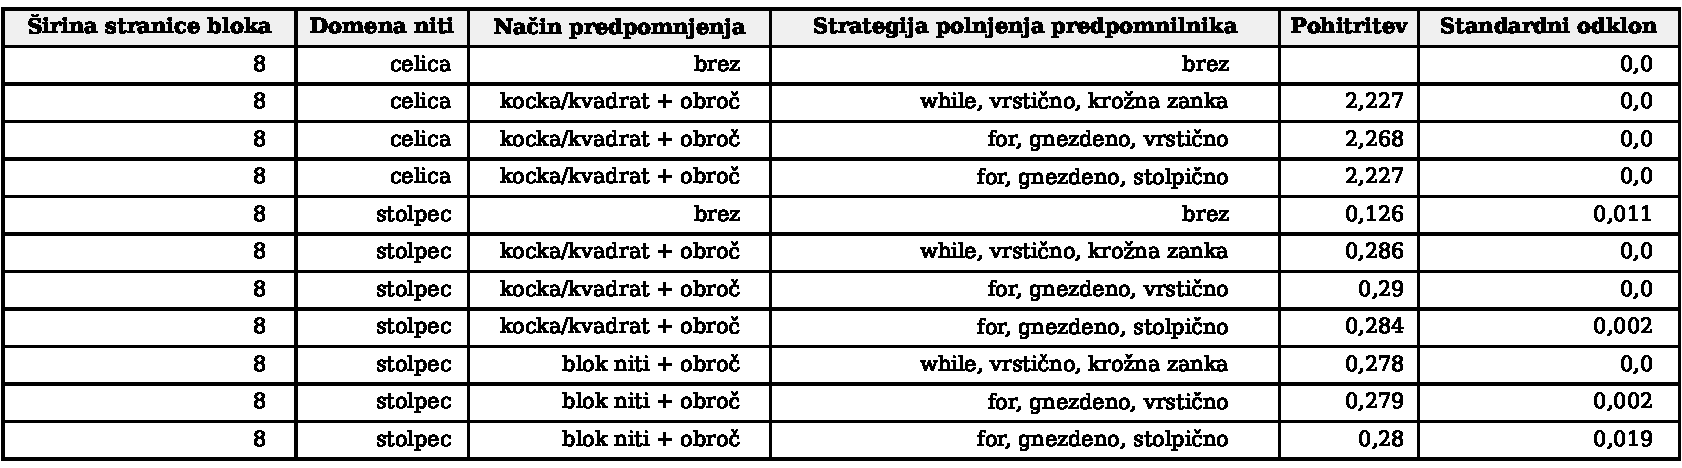
\includegraphics[width=0.9\linewidth]{tables/3D_I1_B8.pdf}
    \label{tab:3D_I1_B8}
\end{table}

\chapter{Zaključek}

Raziskovanje zmogljivosti različnih načinov optimizacije aplikacij z vzorcem matrice je prineslo več vzpodbudnih rezultatov.
Pojavili so se tudi nepričakovani rezultati, ki jih nismo znali pojasniti.

% Povzetek
Iz rezultatov za 2D mrežo lahko zaključimo, da pri domeni niti ene celice velikost bloka ni vplivala na hitrosti izvajanj.
V vseh primerih so predpomnilne strategije bile hitrejše od tiste brez predpomnenja.
Pri sinhronizaciji mreže preko CPE so bile pohitritve majhne, za razliko od sinhronizacije preko GPE, kjer so bile tudi dvokratne.
Druga strategija polnjenja predpomnilnika se je venomer izkazala za najhitrejšo, vedno je bila rahlo pred prvo strategijo.
Tretja strategija je bila pri sinhronizaciji preko CPE najhitrejša, pri sinhronizaciji preko GPE pa konkretno najpočasnejša. Šele pri slednjem načinu se je pokazala razlika zaradi stolpične logike naslavljanja skupnega pomnilnika.
Pri domeni niti enega stolpca v 2D mreži je vedno prišlo do upočasnitve. Razlog za to je v sedaj premajhnih blokih, ki so manjši od enega snopa (\(8^1\) oziroma \(16^1\) celic).

V 3D mreži so se pri obeh načinih predpomnjenja pojavile omejitve pri velikosti soseščine. Izkazalo se je, da na to vpliva tudi velikost bloka.
Pri predpomnjenju kocke in obroča blokov velikosti \(4^3\) je bila omejitev soseščine R=9, pri večjih blokih \(8^3\) pa R=7.
Omejitev soseščine je bila za eno celico večja pri predpomnjenju bloka niti in obroča, kar je vidno iz primerov, kjer je domena niti en stolpec.

Pri \hfill sinhronizaciji \hfill preko \hfill CPE \hfill je \hfill predpomnjenje \hfill bloka \hfill in  \hfill obroča \hfill bilo \\ pričakovano hitrejše od predpomnjenja kocke in obroča, saj se pri prvi metodi porabi manj skupnega pomnilnika.
Takih razlik pri sinhronizaciji na GPE ni bilo opaziti.

Kot pomembno se je izkazalo razmerje med številom niti v bloku in velikostjo skupnega pomnilnika.
Kjer je blok niti majhen v primerjavi z skupnim pomnilnikom, ima vsaka nit več dela pri njegovem polnjenju, kar lahko negativno vpliva na izvajalni časi.
Tako je videti pri blokih \(4^3\) pri sinhronizaciji preko CPE pri domeni niti ene celice, kjer se je pri predpomnjenju pojavila upočasnitev.
Ko smo blok povečali, se je upočasnitev spremenila v pohitritev.
Pri sinhronizaciji preko GPE se ta težava ni pojavila, saj smo tudi pri manjših blokih opazili pohitritve, kar je lahko predmet nadaljnje raziskave.

Izbira velikosti bloka se je pokazala kot zelo pomembna pri domeni niti enega stolpca.
Povsod, kjer je bila domena niti stolpec in blok niti manjši od enega snopa, je prišlo do pričakovanih upočasnitev, tako v 2D, kot tudi v 3D simulacijah.

V nasprotnem primeru, pri domeni enega stolpca in zadostni velikosti bloka je bilo pričakovati pohitritve.
To pričakovanje je upravičila le konfiguracija z velikostjo bloka \(8^2\) pri sinhronizaciji preko CPE in brez predpomnjenja.
Pri vseh ostalih je bilo opaziti upočasnitve.
Pri soseščini R=7, bloku \(8^2\) in sinhronizaciji na CPE sta oba načina predpomnjenja bila počasnejša kot tisti brez predpomnjenja.
Če upoštevamo, da pri predpomnjenju bloka niti in obroča tu predpomnimo za \((7 \times 2 + 8)^2 \times (7 \times 2 + 1)\) celic, je hitro vidno, da je tudi tu poraba skupnega pomnilnika velika, kar pomeni majhno zasedenost GPE in degradirano zmogljivost.
Za razliko od tega, je pri ostalih primerih, še posebej pri sinhronizaciji preko GPE, potrebno nadaljnje raziskovanje.

V 3D mreži pri domeni niti stolpca, večinoma ni bilo videti pomembnih razlik med strategijami polnjenja predpomnilnika.
Tam kjer so se pokazale, je bila tretja strategija ponavadi tako hitra kakor prva, druga je bila rahlo počasnejša.

Pridobili smo karakteristike parametrov, s katerimi smo testirali simulacije Lenie ter pojasnili njihov vpliv.
Poleg njihovega vpliva, obstaja tudi možnost vpliva na nihanje časov izvajanj simulacij zaradi dejstva, da na Arnesovi gruči pri testiranju simulacij nismo zasedli celotnih vozlišč.
To pomeni, da je lahko poganjanje programske kode drugih uporabnikov na istem vozlišču vplivalo na hitrost delovanja naših aplikacij.

Sinhronizacija mreže preko GPE nas je zaradi omejitev strojne opreme prisilila v uporabo relativno majhnih mrež.
To za simulacije realnih problemov predstavlja težavo zaradi višjedimenzionalnih in velikih mrež, zato ta metoda sinhronizacije mreže ni videti ustrezna.

% time tiling predlog
Nekateri avtorji \cite{holewinski2012high, SCHAFER20112027} so uporabili pristop, kjer so v vsaki iteraciji simulacije izračunali stanja več časovnih korakov hkrati, brez potrebe po sinhronizaciji mreže preko CPE.
Tak pristop bi bilo zanimivo preizkusiti v nadaljnjih raziskavah.

% Izbira domena niti stolpca se je izkazala za potencialno dobro, ob predpostavki dovolj velikih blokov niti.
% Število niti v vsakem bloku mora namreč biti večkratnik enega snopa.
% V nadaljnjih raziskavah bi blo potrebno izbrati primernejše velikosti blokov niti, da bi maksimizirali učinek iteriranja po z-plosvah.

Različne metode predpomnjenja so nas opozorile na pomembnost omejenosti z velikostjo skupnega pomnilnika.
Da bi pridobili možnost izvajanja simulacij z večjimi soseščinami, bi lahko obstoječe tehnike nadgradili tako, da bi v več delih napolnili skupni pomnilnik in izračunali nova stanja celic ter se s tem izognili omejitvi skupnega pomnilnika.

% Kjer so razmere omogočale, je bilo predpomnjenje bloka niti in obroča hitrejše od predpomnjenja cele kocke in obroča, seveda ob domeni niti enaki stolpcu.
% Pri navadnem primeru ob domeni niti enaki eni celici je po pričakovanjih načeloma bilo predpomnjene hitrejše od naivne implementacije, ob pogoju, da je blok dovolj velik v primerjavi s celotnim volumnom skupnega pomnilnika.
% Vpliv slednjega razmerja bi bilo zanimivo nadalje raziskati, da bi se našel optimum, pri katerem imamo zagotovljeno pohitritev.

Strategije polnjenja skupnega pomnilnika bi bilo prav tako mogoče podrobneje raziskati, sploh, kjer v primerih, ko je bila strategija s stolpično logiko denimo hitrejša od tiste z vrstično.

% Pogosto \hfill je \hfill težko \hfill identificirati, \hfill kaj \hfill privede \hfill do \hfill premajhne \hfill zasedenosti \\ računskih enot, kar načeloma povzroči upočasnitve.
% Orodje, ki bi nam pri tem v prihodnje lahko pomagalo, je orodje za profiliranje programske kode, vključeno v programski ``paket'' Nvidia Nsight.

\printbibliography[heading=bibintoc, title={Literatura}]

\end{document}
